% .:: Laden der LaTeX4EI Formelsammlungsvorlage
\documentclass[fs, footer]{latex4ei}
\usepackage{latex4ei}
\usepackage[european]{circuitikz}

\usepackage{multirow}
\usepackage{kbordermatrix}

% UPDATE WITHOUT CLASS CHANGE
% ----------------------------------------------------------------------

% LastPage
\usepackage{lastpage}

% Allow hyperlinks
	\RequirePackage[pagebackref=true,pdfpagelabels]{hyperref}
	
% Colors
	\RequirePackage{latex4ei/latex4ei_colors}
	\colorlet{col_link}{tum_blue_dark}
	\hypersetup{
	colorlinks=true,
	linkcolor=col_link,
	urlcolor=col_link,
	citecolor=col_link,
}

% set pdfoptions
	\AtBeginDocument{
		\hypersetup{
			pdftitle={Schaltungstheorie},
	        pdfauthor={LaTeX4EI},
	        pdfcreator={LaTeX4EI template (www.latex4ei.de)},
	        pdfkeywords={latex4ei}
	    }
	}

% Date with git commit number
	\newcommand{\themydate}{\today} % Default URL placeholder
	\newcommand{\mydate}[1]{\renewcommand{\themydate}{#1}}	

% Header and Footer
	\RequirePackage{fancyhdr}

	\pagestyle{fancy}
	\fancyhf{}

	\AtBeginDocument{
	\IfFileExists{git.id}{\input{git.id}}{}
	\ifdefined\GitNiceDate\mydate{\GitNiceDate\ (git \GitRevision)}\fi
	\ifdefined\GitIssuesURL
		\ifdefined\setissueslinkurl
		\setissueslinkurl{\GitIssuesURL} % Set the actual URL
		\fi
	\fi
	}
	
% Define Email
	\providecommand{\email}[1]{\href{mailto:#1}{\nolinkurl{#1}}}
	
%
	\fancyfoot[C]{von LaTeX4EI\ -- Mail: \email{info@latex4ei.de}}
	\fancyfoot[R]{Stand: \themydate \qquad \thepage/\pageref{LastPage}}
	\fancyfoot[L]{Homepage: \url{www.latex4ei.de} -- Fehler bitte \emph{sofort} \href{\issueslinkurl}{melden}.}
	
	\renewcommand{\headrulewidth}{0.0pt} %obere Linie ausblenden
	\renewcommand{\footrulewidth}{0.1pt} %obere Linie ausblenden
	
	\newcommand{\issueslinkurl}{https://github.com/latex4ei/Allgemein/issues} % Default URL placeholder
	\newcommand{\setissueslinkurl}[1]{\renewcommand{\issueslinkurl}{#1}}
% ----------------------------------------------------------------------

% Dokumentbeginn
% ======================================================================
\begin{document}

\titlespacing*{\subsubsection} {0pt}{0.5ex}{2.0ex}
\titlespacing*{\subsection} {0pt}{0.5ex}{2.0ex}
\titleformat{\subsubsection}
  {\normalfont\normalsize\bfseries}{\thesubsubsection}{1em}{}
  

% Aufteilung in Spalten
\vspace{-4mm}
\begin{multicols*}{4}
    \fstitle{Schaltungstheorie}

    % -------------------------------------------
    % |         Schaltungstechnik                |
    % ~~~~~~~~~~~~~~~~~~~~~~~~~~~~~~~~~~~~~~~~~~~
    % SECTION ====================================================================================
    \section{Grundlagen}
    % ============================================================================================

    \sectionbox{
        \subsection{Sinus, Cosinus \quad $\sin^2(x) \bs + \cos^2(x) = 1$}
        \setlength{\tabcolsep}{4pt}
        \tablebox{
            \begin{tabular*}{\columnwidth}{@{\extracolsep\fill}c|c|c|c|c||c|c|c|c@{}} \ctrule
                $x$ & $0$ & $\pi / 6$ & $\pi / 4$ & $\pi / 3$ & $\frac{1}{2}\pi$ & $\pi$ & $1\frac{1}{2}\pi$ & $2 \pi$ \\
                $\scriptstyle{ \varphi }$ & $\scriptstyle{0^\circ}$ & $\scriptstyle{30^\circ}$ & $\scriptstyle{45^\circ}$ & $\scriptstyle{60^\circ}$ & $\scriptstyle{90^\circ}$ & $\scriptstyle{180^\circ}$ & $\scriptstyle{270^\circ}$ & $\scriptstyle{360^\circ}$ \\ \cmrule
                $\sin$ & $0$ & $\frac{1}{2}$ & $\frac{1}{\sqrt{2}}$ & $\frac{\sqrt 3}{2}$ & $1$ & $0$ & $-1$ & $0$ \\
                $\cos$ & $1$ & $\frac{\sqrt 3}{2}$ & $\frac{1}{\sqrt 2}$ & $\frac{1}{2}$ & $0$ & $-1$ & $0$ & $1$ \\
                $\tan$ & $0$ & $\frac{\sqrt{3}}{3}$ &    $1$    &    $\sqrt{3}$ & $\pm \infty$ & $0$ & $\mp \infty$ & $0$\\ \cbrule
            \end{tabular*} }
    }

    Verbraucherpfeilsystem: Spannung und Strom sind assoziiert. Positive Leistung bedeutet Leistungsaufnahme oder Verbrauch von Leistung.
    Negative Leistung bedeutet Leistungsabgabe oder Erzeugung von Leistung.\\
    Das Gegenteil wäre das Erzeugersystem.\
    In den meisten Fachgebieten wird im Verbrauchersystem gerechnet.

    \sectionbox{
        \subsection{Begriffserklärung, Glossar}
        \begin{description}%\itemsep0pt
            \item[Zählpfeile:] Zeigen die gemeinsame(assoziierte) Zählrichtung von Stromfluss und Spannungsabfall zwischen zwei Knoten an, unabhängig von den tatsächlichen Richtungen (Vorzeichen).
            \item[Masse (Signale) $\perp$:] Gemeinsamer el. Bezugspunkt mit Potential $0V$
            \item[Erdung (Fehlstrom):] Schutz vor Kurzschluss, führt nur im Fehlerfall Strom.
            \item[Kurzschluss (KS):] ideal leitender Draht. $u_{\ir KS} = 0$, $i_{\ir KS}=\; \mathrm{beliebig}$
            \item[Leerlauf (LL):] ideal isolierende Luft. $u_{\ir LL}=\; \mathrm{beliebig}$, $i_{\ir LL} = 0$
            \item[Tor:] Ein Tor bilden zwei Anschlüsse bei denen der Stromzufluss des einen Anschluss gleich dem Stromabfluss des anderen Anschluss entspricht. $i_{\ir in} = i_{\ir out}$
            \item[Arbeitspunnkt (AP):] Betriebspunkt bei dem alle Kleinsignalquellen Null sind.
        \end{description}
    }

    % SECTION ====================================================================================
    \section{Netzwerktheorie}
    % ============================================================================================

    \sectionbox{

        \subsection{Kirchhoff-Gesetze}
        Konzentriertheitshypothese: $d \ll \lambda$ mit \\
        $d = $ Größe der Schaltung, Wellenlänge $\lambda = c T$ \\

        %Knotenregel \emph{KCL}: $ \sum \limits_{\text{Knoten}}i_{\ir j} (t) = 0$ (heraußfließende Ströme positiv) \\
        %Maschenregel \emph{KVL}: $ \sum \limits_{\text{Umlauf}} u_{\ir j} (t) = 0$ (Spannungen in Umlaufrichtung positiv)

        \tablebox{
            \begin{tabular*}{\columnwidth}{@{\extracolsep\fill}ll@{}} \trule
                $\underset{\text{Kirchoff's Current Law}}{\text{\large Stromgesetz \textbf{KCL}}}$ & $\underset{\text{Kirchoff's Voltage Law}}{\text{\large Spannungsgesetz \textbf{KVL}}}$ \\ \mrule
                Knotenregel & Maschenregel\\[0.5em]
                $\displaystyle \sum\limits_{\ir Knoten} i_k (t) = 0 $ & $\displaystyle \sum\limits_{\ir Masche} u_m (t) = 0 $ \\[1.5em]
                % ToDo: Bild!!
                rausfließende Ströme positiv & Spannungen in Umlaufrichtung positiv \\
                Maxwell: $\mathrm{div}\, \vec j = 0$ & Maxwell: $\mathrm{rot}\, \vec E = 0$ \\
                $(n-1)$ Gleichungen & $b-(n-1)$ Gleichungen\\ \brule
            \end{tabular*}
        }

    }

    \sectionbox{
        \subsection{Schaltung und Netzwerkgraph}
        % Verbindet man mehrere Bauelemente zu einer Schaltung ergibt sich eine eindeutige Verbindungsstruktur.\\
        Der gerichtete Netzwerkgraph stellt die Verbindungsstruktur einer Schaltung durch $n$ Knoten (node) und $b$ Verbindungskanten (branch) mit Richtungspfeilen dar.\\
        Jedes Bauelement mit zwei Anschlüssen entspricht einer Verbindungskante. Ein Knoten ist dort, wo ein oder mehr Anschlüsse von Bauteilen durch ideal leitenden Draht miteinander verbunden sind.
        Verbundene Anschlüsse entsprechen einem Kurzschluss, nicht verbundene Anschlüsse einem Leerlauf!


        Um die Betriebspunkte einer Schaltung zu bestimmen sind $2b$ linear unabhängige Gleichungen nötig. Man erhält diese $2b$ Gleichungen aus den Beschreibungen der Bauelemente und den Kirchoff Gleichungen.


    }

    \sectionbox{
        \subsection{Baumkonzept}
        \textbf{Baum}: zusammenhängender azyklischer Teilgraph des Netzwerkgraphen, der alle Knoten enthält.\\
        \textbf{Nummerierung}: erst Baumkanten nummerieren, dann übrige.\\
        \textbf{KVL}: Pro Verbindungskante eine Masche, die sonst nur Baumkanten enthält:    $\mat{\ma B_b& \ma 1_s}\mat{\vec u_b\\ \vec u_v} = \vec{0}$\\
        \textbf{KCL}: Pro Baumkante je einen Superknoten, der sonst nur Verbindungskanten enthält, Vorzeichen der Baumkante ist positiv: $\mat{\ma 1_{n-1}&\ma A_v}\mat{\vec i_b\\ \vec i_v} = \vec 0$
    }

    \sectionbox{
        \subsection{Knoteninzidenzmatrix}
        Knoteninzidenzmatrix: $\ma A = \mat{\alpha_{11} &  \ldots & \alpha_{1b} \\ \vdots & &  \\ \alpha_{n-1,1} & \ldots & \alpha_{n-1,b}}$ \quad$n$ Knoten\\
        \textbf{Aufstellen}
        \begin{itemize}\itemsep0pt
            \item Wählen des Bezugsknotens
            \item Für alle Knoten außer Bezugsknoten:
            \item[-] Herausgehende Kante $\Rightarrow \alpha = +1$
            \item[-] Hereingehende Kante $\Rightarrow \alpha = -1$
        \end{itemize}
        KCL: $\ma A \vec i = \vec 0$\quad
        KVL: $\vec u = \ma A^T\vec u_k$
    }

    \sectionbox{
        \subsection{Eintorverschaltungen}
        \tablebox{
            \begin{tabular*}{\columnwidth}{@{\extracolsep\fill}ll@{\hspace{1em}}|ll@{}} \ctrule
                \multicolumn{2}{c}{\large{Serienschaltung}} & \multicolumn{2}{c}{\large{Parallelschaltung}} \\ \ctrule
                $u= \sum u_i$ & $i=\const$ & $u =\const$ & $i=\sum i_i$\\
                $q= \const$ & $\Phi_{\ir M} =\sum \Phi_{{\ir M,}i}$  & $q=\sum q_i$ & $\Phi_{\ir M}=\const$\\ \cmrule
                $R=\sum R_i$ & $M=\sum M_i$ & $\frac{1}{R} = \sum \frac{1}{R_i}$ & $\frac{1}{M} = \sum \frac{1}{M_i}$\\[0.5em]
                $\frac{1}{C} = \sum \frac{1}{C_i}$ & $L=\sum L_i$ & $C=\sum C_i$ & $\frac{1}{L} = \sum \frac{1}{L_i}$ \\[0.5em] \cmrule
                $\cx Z=\sum \cx Z_i$ & $\frac{1}{\cx Y} = \sum \frac{1}{\cx Y_i}$ & $\frac{1}{\cx Z} = \sum \frac{1}{\cx Z_i}$ & $\cx Y=\sum \cx Y_i$\\ \cbrule
            \end{tabular*} }

        \emphbox{$\frac{1}{R} = \frac{1}{R_1} + \frac{1}{R_2} \quad \Ra \quad R = R_1 \parallel R_2 = \frac{R_1 \cdot R_2}{R_1 + R_2}$}
    }

    \sectionbox{
        \subsection{Resistive Eintore}

        \begin{itemize}
            \item Implizite Darstellung: $f_{\mathcal F} (u,i) = 0$
            \item Parameterdarstellung: $u = u_{\mathcal F} ( \lambda )$ \quad $ i = i_{\mathcal F} (\lambda )$
            \item Explizite Darstellung: $\underset{\ir Leitwertdarstellung}{i = g_{\mathcal F} (u)}$ \quad $\underset{\ir Widerstandsdarstellung}{u = r_{\mathcal F} (i)}$
            \item Umpolung: $\overline {\mathcal F}$ entsteht durch Punktspiegelung von $\mathcal F$ am Ursprung: $(\overline u, \overline i) = (- u, - i) \in \overline {\mathcal F}$
            \item Dualität: $(u,i) \in \mathcal F \Leftrightarrow ( R_d i, \frac{ u}{ R_d}) \in {\mathcal F}^d$
            \item Parallelschaltung von Widerstandsgeraden: $G = G_1 + G_2$ \\
                  $\Ra \frac 1 R = \frac 1 R_1 + \frac 1 R_2 \Ra R = R_1 \parallel R_2 = \frac{R_1 R_2}{R_1 + R_2}$
            \item Serienschaltung von Widerstandsgeraden: genauso wie Parallelschaltung nur $R$ statt $G$
            \item Arbeitspunkt ermitteln:
                  \begin{enumerate}
                      \item Schaltung aufteilen in Quelle $\mathcal Q$ und Last $\mathcal L$
                      \item Parameterdarstellung $\Ra$ Kennlinien zeichnen
                      \item Lösung: Schnittpunkte der Kennlinien! $\Ra$ ist die Funktion im AP stetig und diff'bar, kann man sie dort \emph{linearisieren}
                  \end{enumerate}
        \end{itemize}

        Eigenschaften von $\mathcal F$:

        \tablebox{
            \begin{tabular*}{\columnwidth}{@{\extracolsep\fill}ll@{}}
                \ctrule
                $\mathcal F$ stromgesteuert & $\exists r_{\mathcal F}(i)$\\
                $\mathcal F$ spannungsgesteuert & $\exists g_{\mathcal F}(u)$\\
                $\mathcal F$ ungepolt & Kennlinie punktsymm. zum Ursprung \\
                $\mathcal F$ aktiv & mind. 1 Pkt. in II. od. IV. Quadr. \\
                $\mathcal F$ verlustfrei & nur auf Koordinatenachsen \\
                $\mathcal F$ quellenfrei & enthält den Ursprung \\
                $\mathcal F$ streng linear & $(ku, ki) \in \mathcal F$ \quad $ (u_1 + u_2, i_1 + i_2) \in \mathcal F$ \\
                $\mathcal F$ stückweise linear & Kennlinie besteht aus linearen Abschnitten\\
                \cbrule
            \end{tabular*}
        }


    }

    \sectionbox{
        \subsection{Dualwandlung}
        $u \rightarrow R_d\cdot i^d$\qquad $i \rightarrow \frac{1}{R_d}\cdot u^d$
        \\
        Im Schaltbild:\\
        $R \rightarrow G = \frac{R}{R_d^2}$\qquad $G \rightarrow R = R_d^2G$
        \\
        Serienschaltung $\leftrightarrow$ Parallelschaltung
    }

    \sectionbox{
    \subsection{Teilerregeln}
    \textbf{Spannungsteiler}: $R_1$ in Serie mit $R_2$ $\Rightarrow$ $u_{R_1} = \frac{R_1}{R_1+R_2}u_{ges}$\\
    \textbf{Stromteiler}: $G_1$ in Serie mit $G_2$ $\Rightarrow$ $i_{G_1} = \frac{G_1}{G_1+G_2}i_{ges}$
    }

    \sectionbox{
        \subsection{Arbeitspunktbestimmung}
        $\mathcal Q$: Quelleneintor\\
        $\mathcal Q^x$: Quelleneintor mit externer Kennlinie (gespiegelt an der u-Achse)\\
        $\mathcal F$: Lasteintor\\
        \textbf{Graphisch}: $AP = \mathcal F \cap \mathcal Q^x$\\
        \textbf{Rechnerisch}:
        $\begin{array}{l}
                i_Q = -i_{\mathcal F} \Rightarrow u_{AP} \\
                u_Q = u_{\mathcal F} \Rightarrow i_{AP}
            \end{array}$
    }

    % SECTION ====================================================================================
    \section{Resistive Eintore}
    % ============================================================================================

    \sectionbox{
        \subsection{Kennlinienbestimmung von verschalteten Bauteilen}
        \textbf{Parallel}: Kennlinien entlang der i-Achse addieren (Spannungen sind gleich, Ströme addieren sich\\
        \textbf{Seriell}: Kennlinien entlang der u-Achse addieren (Ströme sind gleich, Spannungen addieren sich
    }

    \sectionbox{
    \subsection{Linearisierung}
    Beispiel spannungsgesteuert, stromgesteuert analog\\
    $g_{\text{lin}} = \left. \frac{\partial i_{\mathcal F}}{\partial u_{\mathcal F}} \right|_{AP}$\\
    $\Delta i = i - I_{AP}$ \quad $\Delta u = u - U_{AP}$\\
    $\Delta i = g_{\text{lin}} \Delta u$\\
    $i_{\mathcal F,\text{lin}} = \Delta i + I_{AP} = \Delta u \cdot g_{\text{lin}} + U_{AP} = g_{\text{lin}}(u_{\mathcal F} - U_{AP}) + I_{AP}$
    }

    \sectionbox{
        \subsection{Quellwandlung}
        Lineare Quellen lassen sich ineinander umwandeln.\\
        \begin{center}
        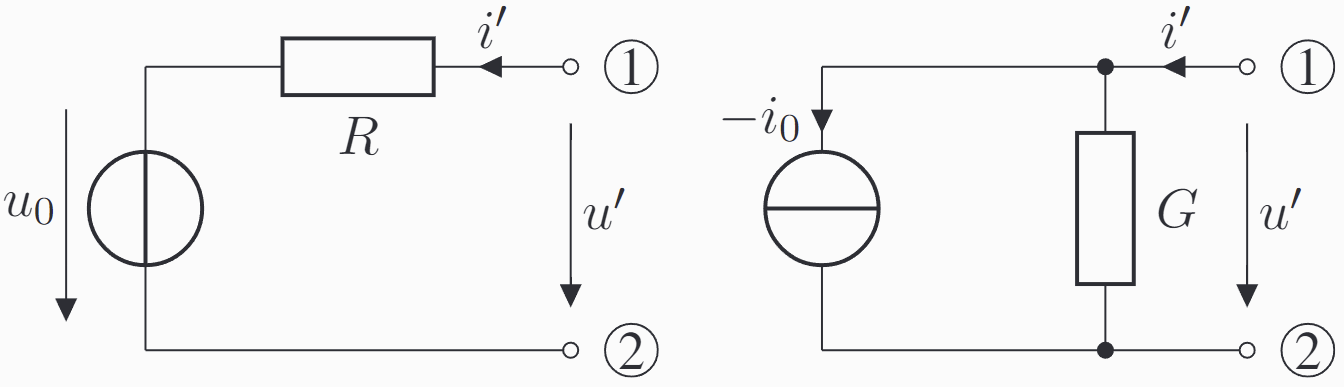
\includegraphics[width=6cm]{./img/source_conv.png}
        \end{center}
        $$i_0=\frac{u_0}R=u_0\cdot G\qquad u_0=\frac{i_0}{G}=i_0\cdot R \qquad R=\frac1G \qquad G= \frac 1R$$

        \textbf{Achtung}: Beachte die umgekehrte Richtung des Stromes $i_0$!
    }

    \subsection{Liste}
    \begin{tabular}{@{}p{1.1cm}p{2.9cm}l}
        \parbox{1.3cm}{ Leerlauf     \\[5pt] \includegraphics{./img/opencircuit.pdf} } & \parbox{2.5cm}{$u=\mathrm{beliebig}$ \\ $i=0$ \\ u, sl, v} & \parbox{1.8cm}{\includegraphics{./img/char/char_opencircuit.pdf} }  \\ \mrule
        \parbox{1.3cm}{ Kurzschluss  \\[5pt] \includegraphics{./img/shortcircuit.pdf}  } & \parbox{2.5cm}{$u = 0$ \\ $i = \mathrm{beliebig}$ \\ u, sl, v} & \parbox{1.8cm}{ \includegraphics{./img/char/char_shortcircuit.pdf} } \\    \mrule
        \parbox{1.3cm}{ Nullator     \\[5pt] \includegraphics{./img/symb/symb_nullator.pdf} } & \parbox{2.5cm}{$u = 0 \quad i = 0$ \\ u, sl, v, dual zu sich selbst} & \parbox{1.8cm}{\includegraphics{./img/char/char_nullator.pdf} } \\ \mrule
        \parbox{1.3cm}{ Norator      \\[5pt] \includegraphics{./img/symb/symb_norator.pdf} } & \parbox{2.5cm}{$u = \mathrm{beliebig}$ \\ $i=\mathrm{beliebig}$ \\[0.5em] u, sl, a, dual zu sich selbst} & \parbox{1.8cm}{\includegraphics{./img/char/char_norator.pdf} } \\ \mrule
        \parbox{1.3cm}{ Widerstand   \\[5pt] \includegraphics{./img/symb/symb_resistor.pdf} }& $\begin{array}{@{}cc} u = R \cdot i \\ i = G \cdot u \end{array} \quad G = \frac{1}{R}$ & \parbox{1.8cm}{\includegraphics{./img/char/char_resistor.pdf} } \\ \mrule
        \parbox{1.3cm}{ \shortstack{Konkaver\\Widerstand}   \\ 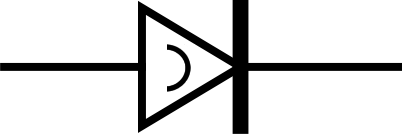
\includegraphics{./img/symb/symb_resistor_concave.png} }& $i=\begin{cases}0&\text{, }u\le U\\ G(u-U)&\text{, }u>U\end{cases}$ & \parbox{1.8cm}{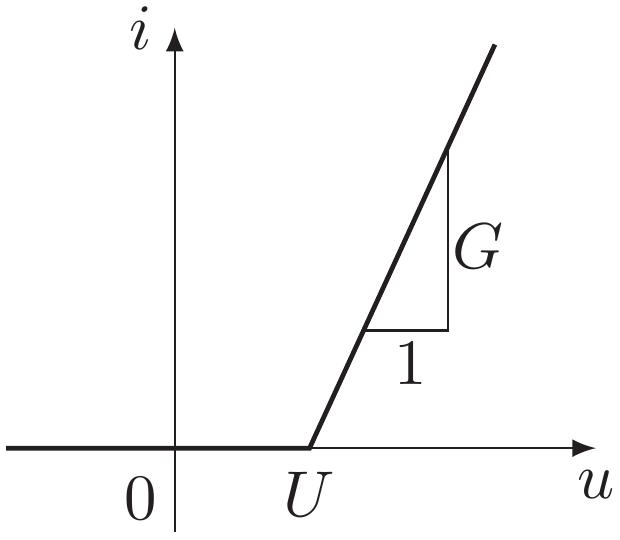
\includegraphics[width=1.8cm]{./img/char/char_resistor_concave.png} } \\ \mrule
        \parbox{1.3cm}{ \shortstack{Konvexer\\Widerstand}   \\ 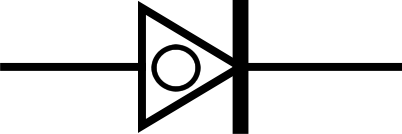
\includegraphics{./img/symb/symb_resistor_convex.png} }& \shortstack{ \shortstack{Dual zum\\\textbf{konkaven Widerstand}} \\ $u=\begin{cases}0&\text{, }i\le I\\ R(i-I)&\text{, }i>I\end{cases}$ }& \parbox{1.8cm}{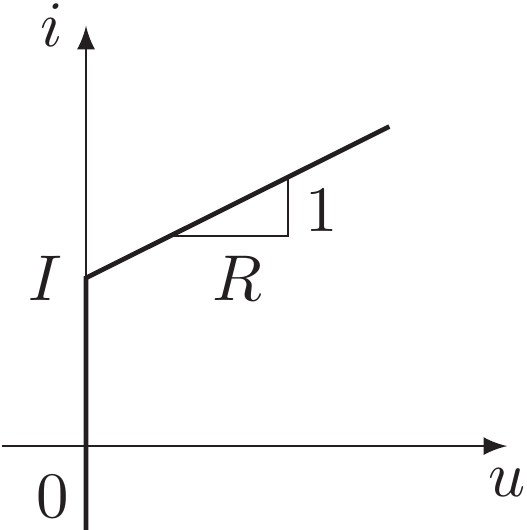
\includegraphics[width=1.6cm]{./img/char/char_resistor_convex.png} } \\ \mrule

        \parbox{1.3cm}{ Spannungsq.  \\[3pt] \includegraphics{./img/symb/symb_source_voltage.pdf} }& $\begin{array}{@{}ll} u = U_0 \\ i = \mathrm{beliebig}\end{array}$ & \parbox{1.8cm}{\includegraphics{./img/char/char_source_voltage.pdf} } \\ \mrule
        \parbox{1.3cm}{ Stromquelle  \\[3pt] \includegraphics{./img/symb/symb_source_current.pdf} }& $\begin{array}{@{}ll} u = \mathrm{beliebig} \\ i = I_0 \end{array}$ & \parbox{1.8cm}{\includegraphics{./img/char/char_source_current.pdf} }    \\ \mrule
        \parbox{1.3cm}{ ideale Diode \\[5pt] \includegraphics{./img/symb/symb_diode.pdf} }& $\begin{array}{@{}ll} u = 0 & \text{falls } i > 0 \\ i = 0 & \text{falls } u < 0\end{array}$ & \parbox{1.8cm}{\includegraphics{./img/char/char_diode_ideal.pdf} } \\ \mrule
        \parbox{1.3cm}{ \shortstack{reale Diode\\pn Diode}  \\[5pt] \includegraphics{./img/symb/symb_diode_real.pdf} }& $\begin{array}{@{}ll} u_D = u_T \cdot \ln \left(\frac{i_D}{I_S} + 1 \right) \\[0.7em] i_D = I_S \cdot \left( \exp \left(\frac{u_D}{U_T}\right) -1 \right) \end{array}$ & \parbox{1.8cm}{\includegraphics{./img/char/char_diode_real.pdf} } \\ \mrule
        \parbox{1.3cm}{ Photodiode   \\ \includegraphics{./img/symb/symb_diode_photo.pdf} }& $i = I_{\ir S} \left( e^{\frac{u_{\ir D}}{U_{\ir T}}} -1 \right) - i_L$ & \parbox{1.8cm}{\includegraphics{./img/char/char_diode_photo.pdf} } \\ \mrule
        \parbox{1.3cm}{ Zenerdiode   \\ 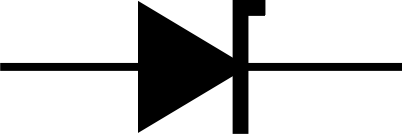
\includegraphics{./img/symb/symb_diode_zener3.png} }& Durchbruch bei $u<U_Z\le 0$: im \textbf{negativen Bereich} leitend & \parbox{1.8cm}{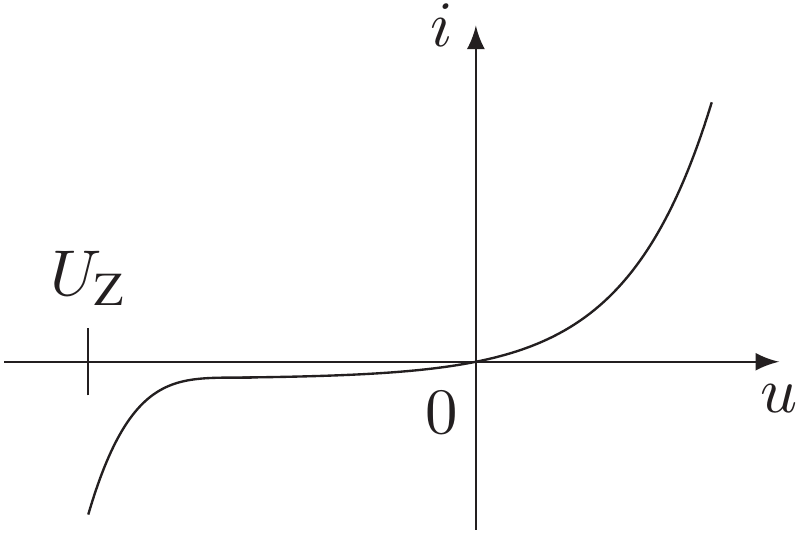
\includegraphics[width=1.8cm]{./img/char/char_diode_zener.png} } \\ \mrule
        \parbox{1.3cm}{ Tunneldiode   \\ 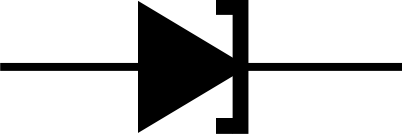
\includegraphics{./img/symb/symb_diode_tunnel2.png} }& \shortstack{Im gewissen Bereich wie ein\\\textbf{negativer Widerstand}} & \parbox{1.8cm}{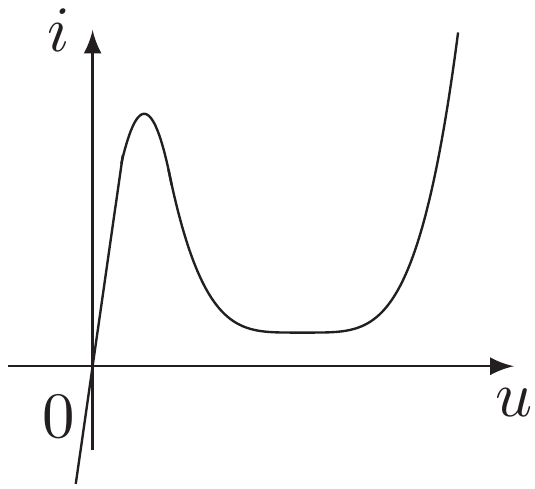
\includegraphics[width=1.7cm]{./img/char/char_diode_tunnel.png} }
    \end{tabular}

    \columnbreak
    % SECTION ====================================================================================
    \section{Resistive Zweitore}
    % ============================================================================================
    Ein Zweitor besteht aus zwei Eintoren.\\

    \subsection{Beschreibungsformen von Zweitoren}
    \begin{tabular}{@{}p{1.3cm}|ll@{}}
        Beschreibung                & nicht linear                                   & linear                                 \\ \mrule
        \textbf{Implizit}           & $f_{\mathcal F}( \ul u, \underline i) = \ul 0$ & $\mat{ \ma M & \ma N} \cdot \mat{\ul u \\ \ul i} = 0$ \\ \mrule
        \textbf{Parametrisch}       & $\begin{array}{@{}l} \ul u = u_{\mathcal F}(\ul \lambda) \\ \ul i=i_{\mathcal F}(\ul \lambda) \end{array}$                   & $\mat{ \ul u                           \\ \ul i } = \mat{\utilde{ \bf U} \\ \utilde{ \bf I}} \cdot \ul \lambda$  \vspace{2em} \\
        \textbf{Explizit}           & nicht linear                                   & linear                                 \\\mrule
        Widerstand-beschreibung     & $\mat{ u_1                                                                              \\ u_2} = \mat{ r_1(i_1,i_2)\\ r_2(i_1,i_2) }$ & $= \mat{ U_0 \\ U_0} + \utilde{ \bf R} \mat{ i_1 \\ i_2} $ \\ \mrule
        Leitwert-beschreibung       & $\mat{ i_1                                                                              \\ i_2} = \mat{g_1(u_1,u_2) \\ g_2(u_1,u_2)}$ & $= \mat{ I_0 \\ I_0} + \utilde{ \bf G} \mat{ u_1 \\ u_2} $ \\ \mrule
        Hybrid-beschreibung         & $\mat{ u_1                                                                              \\ i_2} = \mat{h_1(i_1,u_2) \\ h_2(i_1,u_2)} $ & $= \ma{H} \cdot \mat{ i_1\\ u_2 }$\\ \mrule
        Inver. Hybrid- beschreibung & $\mat{ i_1                                                                              \\ u_2} = \mat{h'_1(u_1,i_2) \\ h'_2(u_1,i_2)}$ & $= \ma{H'} \cdot \mat{ u_1\\ i_2 }$ \\ \mrule
        Ketten-beschreibung         & $\mat{ u_1                                                                              \\ i_1} = \mat{a_1(u_2,-i_2) \\ a_2(u_2,-i_2)}$ & $= \ma{A} \cdot \mat{ u_2\\ -i_2 }$\\ \mrule
        Inver. Ketten- beschreibung & $\mat{ u_2                                                                              \\ i_2} = \mat{a'_1(u_1,-i_1) \\ a'_2(u_1,-i_1)}$ &  $= \ma{A'} \cdot \mat{ u_1\\ -i_1 }$
    \end{tabular}\\

    \subsection{Aufstellen der Zweitormatrix}
    \subsubsection{By Inspection}
    Gleichungen aufstellen und gesuchte Matrix daraus ableiten.
    \subsubsection{Kurzschluss-Leerlauf-Methode}
    Für jede steuernde Größe:
    \begin{itemize}
        \item steuernde Größe einprägen
        \item restliche steuernde Größen auf 0 setzen (mit KS oder LL)
        \item gesteuerte Größen ermitteln
    \end{itemize}
    \subsubsection{Quellenbehaftete lineare Zweitore}
    \begin{enumerate}\itemsep0pt
        \item Matrix des quellenfreien Zweitors bestimmen
        \item Quellvektor bestimmen (beide steuernden Größen auf null setzen)
        \item Schaltbild mit externen Quellen zeichnen je nach Beschreibungsform
    \end{enumerate}



    \subsection{Verschaltung von Zweitoren}
    % ============================================================================================================
    Es gibt sechs mögliche Verschaltungen.\\
    \begin{tabular}{@{}ll}
        Verschaltung & Bild                                                        \\ \hline
        \parbox{3cm}{Parallel: $g_{ges}=g_{\mathcal F1}+g_{\mathcal F2}$           \\ linear: $\ma G_{\ir ges} = \ma G_1 + \ma G_2$ \\ Umrechnung: } & \parbox{2.5cm}{\includegraphics{./img/ztv_leitwert.pdf}}\\[2em]
        \parbox{3cm}{Serie: $r_{ges}=r_{\mathcal F1}+r_{\mathcal F2}$              \\ linear: $\ma R_{\ir ges} = \ma R_1 + \ma R_2$} & \parbox{2.5cm}{\includegraphics{./img/ztv_widerstand.pdf}}\\[2em]
        \parbox{3cm}{Hybrid: $h_{ges}=h_{\mathcal F1}+h_{\mathcal F2}$             \\ linear: $\ma H_{\ir ges} = \ma H_1 + \ma H_2$} & \parbox{2.5cm}{\includegraphics{./img/ztv_hybrid.pdf}}\\[2em]
        \parbox{3.5cm}{Hybrid Inv.: $h'_{ges}=h_{\mathcal F1}+h'_{\mathcal F2}$    \\ linear: $\ma H'_{\ir ges} = \ma H'_1 + \ma H'_2$} & \parbox{2.5cm}{\includegraphics{./img/ztv_hybrid_inv.pdf}}\\[2em]
        \parbox{3cm}{Kette: $a_{ges}=a_{\mathcal F1} \cdot a_{\mathcal F2}$        \\ linear: $\ma A_{\ir ges} = \ma A_1 \cdot \ma A_2$} & \parbox{2.5cm}{\includegraphics{./img/ztv_kette.pdf}}\\[2em]
        \parbox{3cm}{Kette Inv: $a'_{ges}=a'_{\mathcal F2} \cdot a'_{\mathcal F1}$ \\ linear: $\ma A'_{\ir ges} = \ma A'_2 \cdot \ma A'_1$} & \parbox{2.5cm}{\includegraphics{./img/ztv_kette_inv.pdf}}\\
    \end{tabular}

    \subsection{Liste von Zweitoren}
    \subsubsection{VCCS}
    $\ma A = \mat{0&-\frac{1}{g}\\0&0}$\quad
    $\ma G = \mat{0&0\\g&0}$
    \subsubsection{CCCS}
    $\ma A = \mat{0&0\\0&-\frac{1}{\beta}}$\quad
    $\ma H = \mat{0&0\\\beta&0}$
    \subsubsection{VCVS}
    $\ma A = \mat{\frac{1}{\mu}&0\\0&0}$\quad
    $\ma H' = \mat{0&0\\\mu&0}$
    \subsubsection{CCVS}
    $\ma A = \mat{0&0\\\frac{1}{r}&0}$\quad
    $\ma R = \mat{0&0\\r&0}$

    \subsubsection{Nullor}
    $\ma A = \mat{0&0\\0&0}$\quad
    $\ma M = \mat{1&0\\0&0}$\quad
    $\ma N = \mat{0&0\\1&0}$\\
    Eigenschaften: Quellenfrei, streng linear

    \subsubsection{Übertrager (z.B. Transformator)}
    $A=\begin{bmatrix} \text{ü} & 0 \\ 0 & \frac{1}{\text{ü}} \end{bmatrix}$\\
    $R_{in}=\frac{u_1}{i_1}=\text{ü}^2 R_L$\\
    Eigenschaften: verlustlos(ideal)


    \subsubsection{Gyrator}
    Der Gyrator wandelt das an Tor 1 geschaltete Bauteil in das duale Bauteil an Tor 2 um.\\
    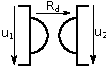
\includegraphics[scale=.8]{./img/symb/symb_gyrator.pdf}
    $\begin{array}{l}
            \ma A=\mat{0 & R_d \\ \frac{1}{R_d} & 0}\mathrm{\quad}\ma R = \mat{0&-R_d\\R_d&0}\\ \mathrm{\quad} G = \mat{0&G_d\\-G_d&0}\mathrm{\quad}\mathcal F_{in}=\mathcal F^d
        \end{array}$\\
    Eigenschaften: streng linear, verlustlos für $R_1=R_2$\\

    \subsubsection{Negativ-Immitanz-Konverter}
    $A=\begin{bmatrix} -k & 0 \\ 0 & \frac{1}{k} \end{bmatrix}$\\
    $R_{in}=\frac{u_1}{i_1}=-k^2R$ \quad $-k^2 R:$\ negativer Widerstand(et voilà xD)\\
    Eigenschaften: streng linear, aktiv

    \sectionbox{
        \subsection{NIK allgemein (Polung beachten)}
        \includegraphics[scale = 0.85]{./img/NIK.pdf} \qquad \includegraphics{./img/char/char_NIK.pdf}\\
        \begin{tabular}{cll}
            I   & negative Sättigung $u_d < 0 \Leftrightarrow u_{out}=-U_{sat}$                                  \\
                & $u = R_0 i - U_{sat}$                                                                          \\ % < \frac{R_L}{R_L + R_1} \cdot U_{sat}$\\
            II  & linearer Bereich $u_d = 0$                                                                     \\
                & $u = - \frac{R_0}{R_1} R_L \cdot i$ \qquad \quad $-U_{sat} < \frac{R_L + R_1}{R_L}u < U_{sat}$ \\
            III & positive Sättigung $u_d > 0 \Leftrightarrow u_{out}=U_{sat}$                                   \\
                & $u = R_0 i + U_{sat}$                                                                          % < \frac{R_L}{R_L + R_1} \cdot U_{sat}$\\
        \end{tabular}
    }

    \subsection{Dualwandlung}
    $\mat{\ma U\\\ma I}^d = \mat{R_d\ma I\\\frac{1}{R_d}\ma U}$\\
    $\ma G^d = \frac{1}{R_d^2} \ma R$ \quad $\ma R^d = R_d^2 \ma G$

    \subsection{Linearisierung}
    \begin{tabular}{ll}
        Großsignal                 & Kleinsignal                  \\
        $i=I_{\ir AP}+\Delta i$ \  & \ $\Delta i= i - I_{\ir AP}$ \\
        $u=U_{\ir AP}+\Delta u$ \  & \ $\Delta u= u - U_{\ir AP}$ \\
    \end{tabular}
    \\
    $\vec i = \vec g(\vec u)$\quad$\Delta \vec i \approx \ma G \cdot \Delta \vec u$\\
    $\ma G$ ist die Jakobimatrix $\left. \frac{\partial g_i(\vec u)}{\partial u_j} \right|_{U_{\ir AP}} = \left. \mat{
            \frac{\partial g_1}{\partial u_1} & \frac{\partial g_1}{\partial u_2}\\
            \frac{\partial g_2}{\partial u_1} & \frac{\partial g_2}{\partial u_2}
        }\right|_{U_{AP}}$\\
    $\Delta \vec u \approx \ma R \cdot \Delta \vec u$\\
    Großsignal: $i \approx I_{\ir AP} + G(U_{\ir AP}) \cdot (u - U_{\ir AP})$\\[1em]

    Implizite Linearisierung: $\Delta \vec f(\Delta \vec u, \Delta \vec i) = \ma M \Delta \vec u + \ma N \Delta \vec i$\\
    $\ma M := \mat{ \frac{\partial f_1}{\partial u_1} & \frac{\partial f_1}{\partial u_2} \\[0.5em] \frac{\partial f_2}{\partial u_1} & \frac{\partial f_2}{\partial u_2} }$ \quad
    $\ma N := \mat{ \frac{\partial f_1}{\partial i_1} & \frac{\partial f_1}{\partial i_2} \\[0.5em] \frac{\partial f_2}{\partial i_1} & \frac{\partial f_2}{\partial i_2} }$

    \section{Resistive Mehrtore}
    \subsection{Beschreibungsformen}
    Analog zu Zweitoren, nur mit mehr Dimensionen und es gibt sehr viele, nicht mehr benannte Hybridbeschreibungen.
    \subsection{Spezielle Mehrtore}
    \subsubsection{Mehrtorübertrager}
    $\ma H_{\text{Übertrager}} = \mat{\ma 0 & \ma H_{a,b}\\-\ma H^T_{a,b}&\ma 0}$\\
    $\ma H'_{\text{Übertrager}} = \mat{
            0 & -\frac{1}{"u_2} & -\frac{1}{"u_3} & \cdots & -\frac{1}{"u_p}\\
            \frac{1}{"u_2} & 0 & 0 & \cdots & 0\\
            \frac{1}{"u_3} & 0 & 0 & \cdots & 0\\
            \vdots & \vdots & \vdots & \ddots & \vdots\\
            \frac{1}{"u_p} & 0 & 0 & \cdots & 0}$\\
    Eigenschaften: Verlustlos und Reziprok

    \subsubsection{Zirkulator}
    $\ma M = \ma 1$ \quad $\ma N = \mat{
            0 & -R & +R\\
            +R &  0 & -R\\
            -R & +R &  0}$\\
    $\ma R = -\ma M^{-1}\ma N = -\ma N = \mat{
            0 & +R & -R\\
            -R &  0 & +R\\
            +R & -R &  0} = -\ma R^T$\\
    Eigenschaften: Verlustlos, Nicht reziprok, Schiefsymmetrisch\\
    $p_1 = u_1i_1 = \frac{u_0^2}{4R} \geq 0W$\\
    $p_2 = u_2i_2 = -\frac{u_0^2}{4R} = -p_1 \leq 0W$\\
    $P_3 = u_3i_3 = 0W$\\
    Die an einem Tor aufgenommene Leistung wird in Pfeilrichtung an das nächste weitergegeben.

    \subsubsection{Multiplizierer}
    $\mat{i_1\\i_2\\u_3} = h\left(\mat{u_1\\u_2\\i_3}\right) = \mat{0\\0\\\frac{u_1u_2}{U_M}}$\quad$u_3=\frac{u_1u_2}{U_M}$, $U_M$ Multipliziererkonstante

    \subsubsection{Dividierer}
    $\mat{i_1\\i_2\\u_3} = h\left(\mat{u_1\\u_2\\i_3}\right) = \mat{0\\0\\\frac{u_1}{u_2}U_D}$\quad$u_3=\frac{u_1}{u_2}U_D$, $U_D$ Dividiererkonstante, $U_D = -U_M$\\
    Realisierung z.B. mit Multiplizierer in Rückkopplungspfad von OpAmp.
    % SECTION ====================================================================================
    \section{Eigenschaften von Ein- und Mehrtoren}
    % ============================================================================================
    Ein Mehrtor $\mathcal F(\vec u, \vec i)$ ist ...

    \textbf{Resistiv}: Gedächtnislos; nur von $u$ und $i$ abhängig\\
    \textbf{Zeitvariant}: Betriebsraum kann sich ändern\\
    \textbf{Reziprozität}: $\ma G^T$ = $\ma G$, $\ma R^T$ = $\ma R$, $\det (\ma A)$ = 1, $\det (\ma {A'})$ = 1, $h_{21} = -h_{12}$, $h'_{21} = -h'_{12}$, $\ma U^T\ma I$ = $\ma I^T\ma U$\\
    \textbf{Symmetrie}: $r_{11} = r_{22}$, $\ma R = \ma P\ma R\ma P$, $\ma G = \ma P \ma G \ma P$ mit $\ma P = \mat{0 & 1 \\ 1 & 0}$, $\ma A = \ma A'$

    \tablebox{
        \begin{tabular*}{\columnwidth}{@{\extracolsep\fill}ll@{}}
            \ctrule
            Eigenschaft & Bedingung\\ \mrule
            $\mathcal F$ quellenfrei & $\vec 0 \in \mathcal F$; enthält den Ursprung \\
            $\mathcal F$ streng linear & $(ku, ki) \in F$ \quad $ (u_1 + u_2, i_1 + i_2) \in F$ \\
            \cbrule
            \\
            Nur für Eintore:\\
            ungepolt & Kennlinie punktsymm. zum Ursprung \\
            & $\mathcal F(u,i)=\mathcal F(-u,-i)$
        \end{tabular*}
    }

    \subsection{Linearität}
    Linear: $(ku, ki) \in F$ \quad $(u_1 + u_2, i_1 + i_2) \in F$ (Kennlinie gerade) \\
    Streng Linear: linear + quellenfrei, (Gerade durch Ursprung)\\

    \subsection{Zeitvarianz}
    Ein Mehrtor heißt zeitvariant, wenn sich sein Betriebsraum mit der Zeit ändern kann, ansonsten
    ist es Zeitinvariant.

    \subsection{Steuerung}
    Ein Bauelement ist von einer Größe gesteuert, wenn die jeweilige explizite Beschreibung existiert.\\
    \begin{tabular*}{\columnwidth}{@{\extracolsep\fill}llll@{}}
        Stromgesteuert: & $u=\mathcal R(i)$ & Spannungsgestuert: & $i=\mathcal G(i)$\\
        Ladungsgesteuert: & $u=\mathcal C^{-1}(q)$ & Flussgesteuert: & $i=\mathcal L^{-1}(\Phi)$
    \end{tabular*}

    \subsection{Leistungsbetrachtung}
    Verlustlosigkeit: $\ma U^T\ma I + \ma I^T \ma U = 0$\\
    Leistung: $P(t)=\ul u^T \cdot \ul i=u_1 i_1 + \dotsc + u_n i_n$ \\
    \begin{tabular*}{\columnwidth}{@{\extracolsep\fill}lll@{}}
        Passiv: & $\forall \mathcal F(u,i): P(t)\ge 0$ & Kennlinie nur I. oder III. Quadrant\\
        Aktiv: & $\exists \mathcal F(u,i): P(t)<0$ & Kennlinie im II. oder IV. Quadrant\\
        Verlustlos: & $\forall \mathcal F(u,i): P(t)=0$ & Kennlinie nur auf Koordinatenachsen\\
    \end{tabular*}\\
    Merke: Alle Mehrtore die nur aus passiven Bauelementen(R,C,L,...) bestehen, sind selbst passiv!
    inkremental passiv:\\
    letztendlich passiv: $\exists U,I>0 \ \forall (u,i) \in \mathcal F : (|u| > U \lor |i| > I \ \Rightarrow \ ui > 0)$\\
    Alle realen Bauteile sind letztendlich passiv, da sonst unendlich viel Energie entstehen würde.\\


    % SECTION ====================================================================================
    \section{Allgemeine Analyseverfahren}
    % ============================================================================================

    \subsection{Tellegenscher Satz}
    $u^Ti = 0$\\
    Der Spannungsvektor steht immer senkrecht zum Stromvektor ($\ma A\ma B^T = \vec 0$ bzw. $\ma B\ma A^T = \vec 0$).

    \subsection{Die Tableau-Gleichung}
    ... beschreibt ein Netzwerk vollständig bezüglich Verschaltung und Bauteilverhalten.\\
    $\mat{\ma B&\ma 0\\\ma 0&\ma A\\\ma M & \ma N}\mat{\vec u\\\vec i} = \mat{\vec 0\\\vec 0\\\vec e}$\qquad
    $\ma T = \mat{ \ma B & \ma 0 \\ \ma 0 & \ma A \\ \ma M & \ma N}$\\
    ($e = 0 \Leftrightarrow$ keine Quellen enthalten)

    \subsection{Newton-Raphson-Algorithmus}
    ... ist ein iterativer numerischer Algorithmus zum Suchen der Nullstellen von nichtlinearen Gleichungen. Algorithmus wählt iterativ die Nullstelle der Taylorentwicklung als nächsten Bezugspunkt.\\
    Taylorentwicklung zu 0 setzen: $f(x^{(j)}) + J(x^{(j)})(x^{(j+1)}-x^{(j)})=0$\\
    Iterationsformel: $x^{(j+1)} = x^{(j)} - J^{-1}(x^{(j)})f(x^{(j)})$\\
    1. Wähle Initialisierung $\mat{\vec u^\textbf{(0)}\\\vec i^ \textbf{(0)}}$ mit $\vec f(\vec u^\textbf{(0)}, \vec u^\textbf{(0)}) = \vec{0}$.\\
    2. Im n+1-ten Schritt: Linearisieren $\vec f(\vec u, \vec i) = \vec 0$ im n-ten Kandidaten für den AP $\mat{\vec u^\textbf{(n)}\\\vec i^ \textbf{(n)}}$.\\
    3. Löse das neue lineare Gleichungssystem (z.B. Tableau).\\
    4. Finde neuen Kandidaten für AP in der Nähe $\mat{u^{(n+1)^T}, i^{(n+1)^T}}$ mit $\vec f(\vec u^\textbf{(n+1)}, \vec i^ \textbf{(n+1)}) = \vec 0$.\\
    5. Wiederhole Schritt 2. - 4. bis $\left|\left|\mat{\vec u^\textbf{(n+1)}\\\vec i^ \textbf{(n+1)}}-\mat{\vec u^\textbf{(n)}\\\vec i^ \textbf{(n)}}\right|\right| \leq \epsilon$ (Toleranz/Genauigkeit).


    \subsection{Knotenspannungsanalyse}
    \boxed{ \underset{\text{Knotenleitwertsmatrix}}{\ma Y_{\ir k}} \cdot \underset{\text{Spannungsvektor}}{\vec u_{\ir k}} = \underset{\text{Stromquellenvektor}}{\vec i_{\ir q}} }\\
    Vorgehen:
    \begin{enumerate}\itemsep0pt
        \item Nicht lineare Elemente linearisieren
        \item Nicht spannungsgesteuerte Elemente (dual)wandeln
        \item Aufstellen der Leitwertsmatrix $\ma Y'_k$
        \item Bestimmung des Stromquellenvektors $\vec i'_q$
        \item Einbau des Nullators: Addition der Spalten von $\ma Y'_k$ an denen er anliegt \& eine Spalte streichen
        \item Einbau des Norators: Addition er Zeilen \& eine Zeile streichen

    \end{enumerate}
    Spezialfall: Nullator/Norator mit Masse verbunden: Spalte/Zeile streichen
    \subsubsection{Aufstellen der Knotenleitwertsmatrix}
    \tiny
    \begin{tabular}{ll}
        $\ma {Y_k} = \kbordermatrix{ & \alpha &                                   & \beta                                                                                          &                                  & \gamma                                                                                       \\
        \alpha                       &        &                                   &                                                                                                & \ldots                           & G_d                                                                                          \\
                                     &        &                                   &                                                                                                &                                  & \vdots                                                                                       \\
        \beta                        &        &                                   &                                                                                                & \ldots                           & -G_d                                                                                         \\
                                     & \vdots &                                   & \vdots                                                                                         &                                  & \vdots                                                                                       \\
        \gamma                       & -G_d   & \ldots                            & G_d                                                                                            & \ldots\\}$ & \parbox{3cm}{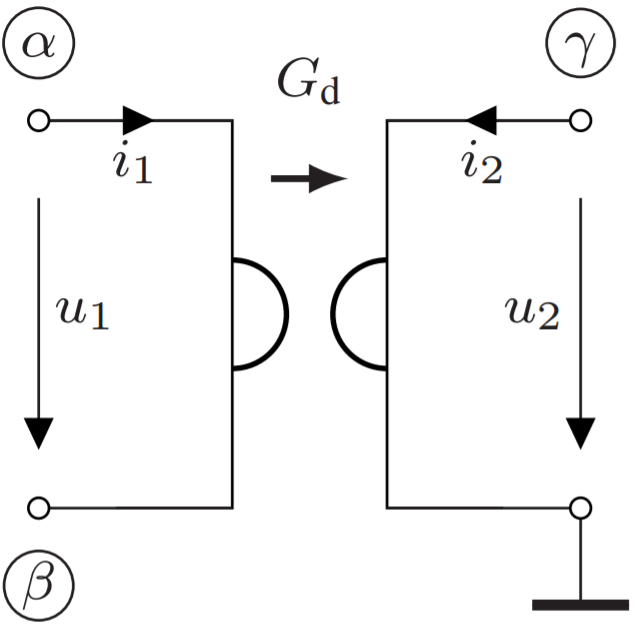
\includegraphics[scale=0.15]{./img/nodevoltageanalysis/gyrator_a_b_y_gnd.png} } \\
        $\ma {Y_k} = \kbordermatrix{ & \alpha &                                   & \gamma                                                                                         &                                  & \delta                                                                                       \\
        \alpha                       &        & \ldots                            & G_d                                                                                            & \ldots                           & -G_d                                                                                         \\
                                     & \vdots &                                   & \vdots                                                                                         &                                  & \vdots                                                                                       \\
        \gamma                       & -G_d   & \ldots                                                                                                                                                                                                                                                               \\
                                     & \vdots                                                                                                                                                                                                                                                                        \\
        \delta                       & G_d    & \ldots \\}$ & \parbox{3cm}{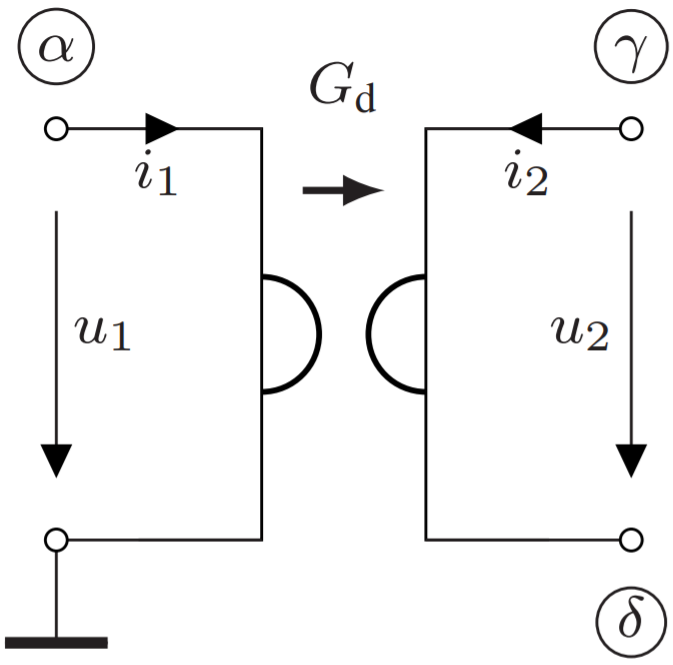
\includegraphics[scale=0.15]{./img/nodevoltageanalysis/gyrator_a_y_d_gnd.png} }                                                                                                                                     \\
        $\ma {Y_k} = \kbordermatrix{ & \alpha &                                   & \gamma                                                                                                                                                                                                                           \\
        \alpha                       &        & \ldots                            & G_d                                                                                                                                                                                                                              \\
                                     & \vdots &                                   & \vdots                                                                                                                                                                                                                           \\
        \gamma                       & -G_d   & \ldots\\}$  & \parbox{3cm}{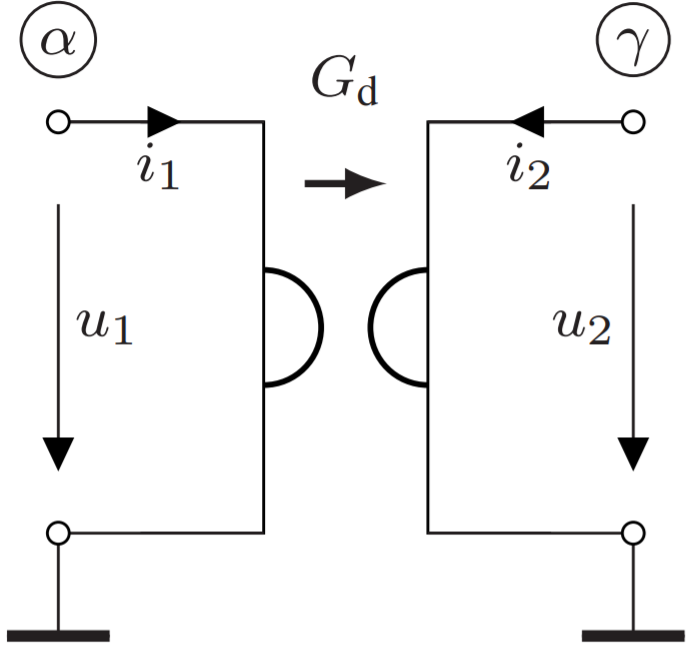
\includegraphics[scale=0.15]{./img/nodevoltageanalysis/gyrator_a_y_gnd_gnd.png} }                                                                                                                                   \\
    \end{tabular}
    $\ \ \ \ \ma {Y_k} = \kbordermatrix{ & \alpha & & \beta & & \gamma & & \delta\\
            \alpha & & & & \ldots & G_d & \ldots & -G_d\\
            & & & & & \vdots & & \vdots\\
            \beta & & & & \ldots & -G_d & \ldots & G_d\\
            & \vdots & & \vdots && \vdots && \vdots\\
            \gamma & -G_d & \ldots & G_d & \ldots\\
            & \vdots & & \vdots\\
            \delta & G_d & \ldots & -G_d & \ldots \\}$ \\
    \begin{center}
        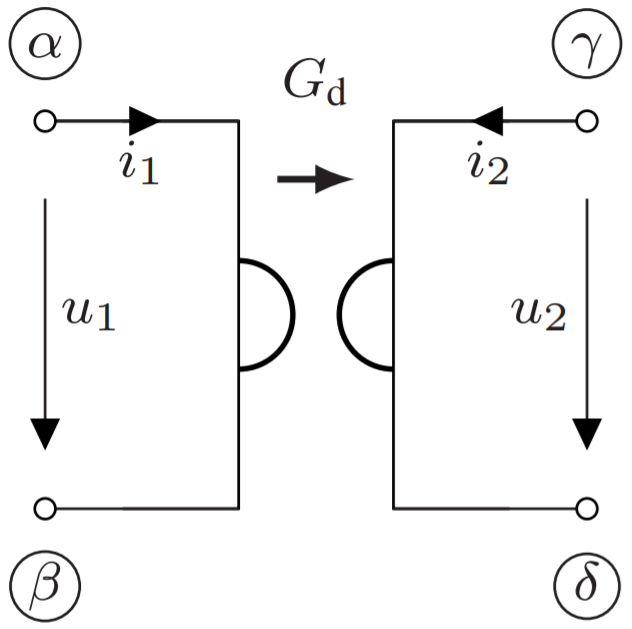
\includegraphics[scale=0.15]{./img/nodevoltageanalysis/gyrator_a_b_y_d.png}
    \end{center}\ \\
    \hrule
    \begin{tabular}{ll}
        $\ \ \ \ \ma {Y_k} = $
        $\kbordermatrix{ &        & \alpha &                            & \beta                                                                                        &                                                                                                                         \\
                         &        & \vdots &                            & \vdots                                                                                       &                                                                                                                         \\
        \alpha           & \ldots & G      & \ldots                     & -G                                                                                           & \ldots                                                                                                                  \\
                         &        & \vdots &                            & \vdots                                                                                       &                                                                                                                         \\
        \beta            & \ldots & -G     & \ldots                     & G                                                                                            & \ldots                                                                                                                  \\
                         &        & \vdots &                            & \vdots                                                                                       & \\}$ & \parbox{3cm}{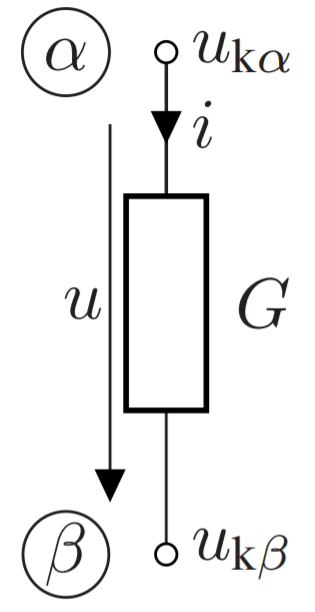
\includegraphics[scale=0.15]{./img/nodevoltageanalysis/conductance_a_b.png} } \\

        $\ \ \ \ \ma {Y_k}$ =
        $\kbordermatrix{ &        & \alpha &                                                                                                                                                                                                                                                     \\
                         &        & \vdots &                                                                                                                                                                                                                                                     \\
        \alpha           & \ldots & G      & \ldots                                                                                                                                                                                                                                              \\
                         &        & \vdots & \\}$ & \parbox{3cm}{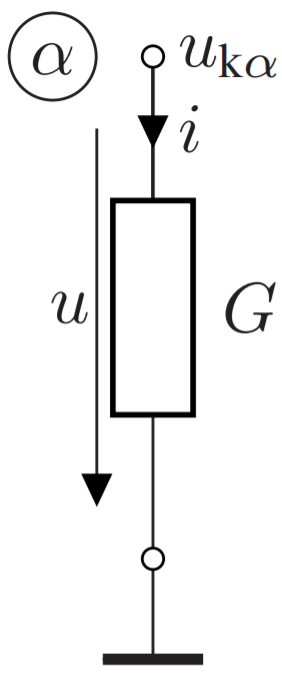
\includegraphics[scale=0.15]{./img/nodevoltageanalysis/conductance_a_gnd.png} }                                                                                                                           \\
    \end{tabular}

    \begin{tabular}{ll}
        $\ \ \ \ \ma {Y_k}$ =
        $\kbordermatrix{ & \gamma &                            & \delta                                                                                                                                                                                                                                       \\
                         & \vdots &                            & \vdots                                                                                                 &                                                                                                                                     \\
        \alpha           & g_m    & \ldots                     & -g_m                                                                                                                                                                                                                                         \\
                         & \vdots &                            & \vdots                                                                                                                                                                                                                                       \\
        \beta            & -g_m   & \ldots                     & g_m                                                                                                                                                                                                                                          \\
                         & \vdots &                            & \vdots                                                                                                 & \\}$ & \hspace{-2em}\parbox{3cm}{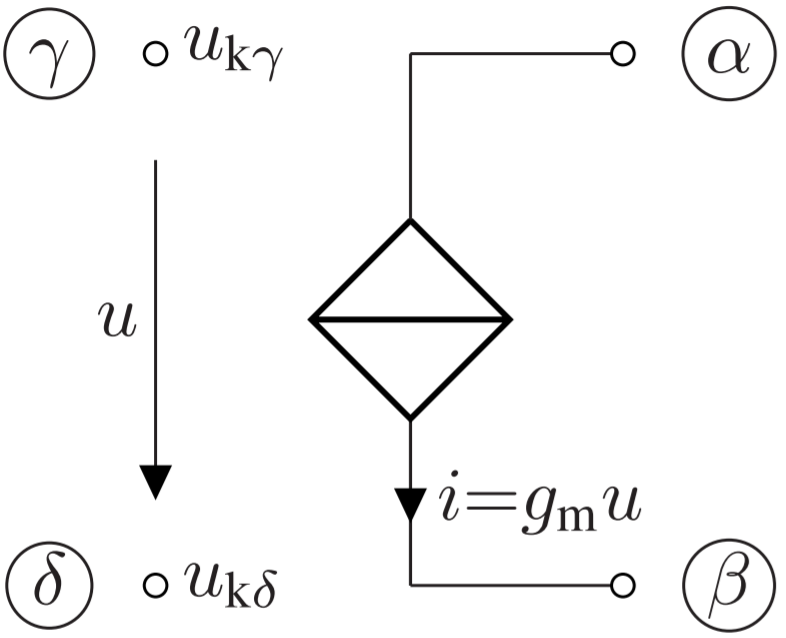
\includegraphics[scale=0.15]{./img/nodevoltageanalysis/vccs_a_b_y_d.png} }   \\

        $\ \ \ \ \ma {Y_k}$ =
        $\kbordermatrix{ & \gamma &                                                                                                                                                                                                                                                                           \\
                         & \vdots &                                                                                                                                                                                                                                                                           \\
        \alpha           & g_m    & \ldots                                                                                                                                                                                                                                                                    \\
                         & \vdots &                                                                                                                                                                                                                                                                           \\
                         & \vdots &                                                                                                                                                                                                                                                                           \\
        \beta            & -g_m   & \ldots                                                                                                                                                                                                                                                                    \\
                         & \vdots & \\}$ & \hspace{-2em}\parbox{3cm}{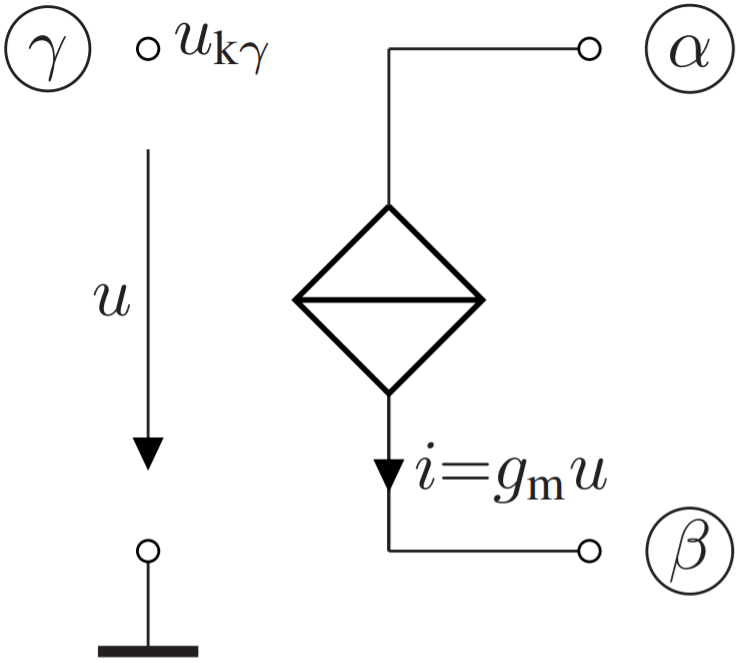
\includegraphics[scale=0.15]{./img/nodevoltageanalysis/vccs_a_b_y_gnd.png} }                                                                                                                                       \\

        $\ \ \ \ \ma {Y_k}$ =
        $\kbordermatrix{ & \gamma &                            & \delta                                                                                                 &                                                                                                                                     \\
                         & \vdots &                            & \vdots                                                                                                 &                                                                                                                                     \\
        \alpha           & g_m    & \ldots                     & -g_m                                                                                                   & \ldots                                                                                                                              \\
                         & \vdots &                            & \vdots                                                                                                 & \\}$ & \hspace{-2em}\parbox{3cm}{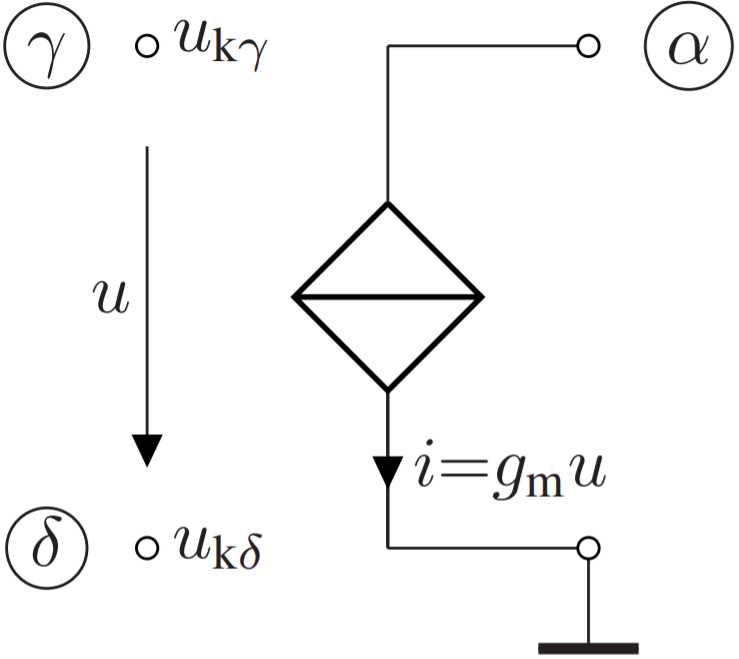
\includegraphics[scale=0.15]{./img/nodevoltageanalysis/vccs_a_y_d_gnd.png} } \\

        $\ \ \ \ \ma {Y_k}$ =
        $\kbordermatrix{ & \gamma &                                                                                                                                                                                                                                                                           \\
                         & \vdots &                                                                                                                                                                                                                                                                           \\
        \alpha           & g_m    & \ldots                                                                                                                                                                                                                                                                    \\
                         & \vdots & \\}$ & \hspace{-2em}\parbox{3cm}{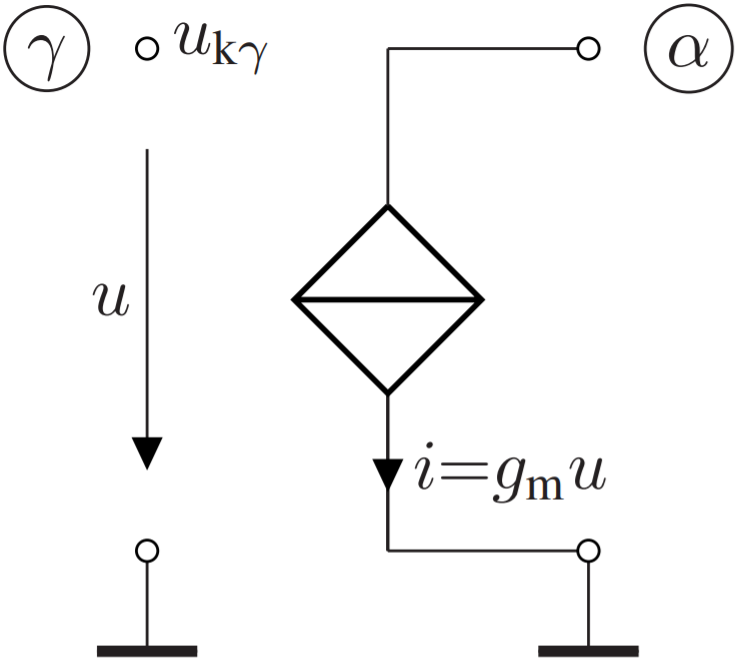
\includegraphics[scale=0.15]{./img/nodevoltageanalysis/vccs_a_y_gnd.png} }                                                                                                                                         \\
    \end{tabular}\\
    \normalsize
    \subsubsection{Aufstellen des Knottenstromquellenvektors}
    Bei dem Vektor $\vec i_{q}$ werden die \textbf{konstanten Quellenströme} eingetragen.
    Anders als üblicherweise, trägt man in der $i$-ten Zeile den Strom $I_0$, der aus dem Knoten \textbf{rausfließt}, \textbf{negativ} ein und den Strom $I_0$, der in den Knoten \textbf{hineinfließt}, \textbf{positiv} ein.\\

    Ist eine Quelle auf einer Seite mit dem Masseknoten verbunden, wird nur der Wert für den gegenüberliegenden (nicht mit Masse verbundenen) Knoten im Stromquellenvektor eingetragen.
    $\vec i_{q} = \mat{0 &\cdots &I_0 &\cdots &0}^T$

    \subsubsection{Berechnen der Knotenspannungen}
    -\ Umformung und Auflösung von $\ma {Y_k} * \vec u_k = \vec i_q$\\
    -\ Cram'sche Regel: $u_{ki} = \frac{\det(\ma Y_{ki})}{\det(\ma Y_k)}$ wobei $\ma Y_{ki}$ durch Ersetzen der i-ten Spalte von $\ma {Y_k}$ mit $\vec i_q$.\\

    \subsection{Dualwandlung}
    $\vec u \xrightarrow{R_d} R_d\vec i^d$\qquad$\vec i \xrightarrow{R_d} \frac{1}{R_d}\vec u^d$\\
    $\ma A\vec i = \vec 0 \xrightarrow{R_d} \ma A\vec u^d = \vec 0$ Knoten werden zu Maschen\\
    $\ma B\vec u = \vec 0 \xrightarrow{R_d} \ma B\vec i^d = \vec 0$ Maschen werden zu Knoten\\
    \begin{tabular}{cc}
        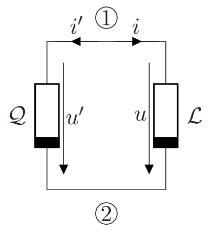
\includegraphics[width=.295\columnwidth]{img/dual_start} &
        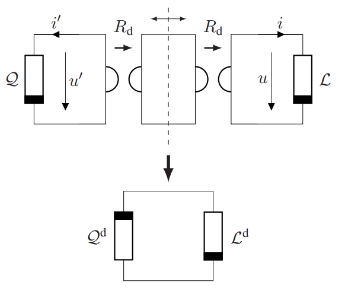
\includegraphics[width=.595\columnwidth]{img/dual_end}
    \end{tabular}
    $\mat{\vec u^d\\\vec i^d}=\mat{0&R_d\\\frac{1}{R_d}&0}\mat{\vec u\\\vec i}$

    \subsection{Substitutionstheorem}
    \includegraphics[scale=.27]{img/subst}\\
    \begin{tabular}{cc}
        \multicolumn{2}{c}{Wenn $\mathcal N_1$ zu allen Zeitpunkten} \\
        spannungsgestuert                        & stromgesteuert    \\
        \includegraphics[scale=.25]{img/subst-u} &
        \includegraphics[scale=.25]{img/subst-i}
    \end{tabular}

    \subsection{Superpositionsprinzip}
    Sei eine lineare eindeutig lösbare Schaltung mit mehreren Erregungen gegeben, so setzt sich die Gesamtlösung aus den einzelnen Teillösungen zusammen.
    \begin{enumerate}\itemsep0pt
        \item Setze alle bis auf eine unabhängige Quelle $U_k$ bzw. $I_k$ zu Null
        \item Berechne die gesuchten Größen $u_{z_k}$ bzw. $i_{y_k}$
        \item Wiederhole Schritte 1 und 2 $\forall$ unabhängige Quellen
        \item Gesamtlösung ergibt sich zu $u_z = \sum_ku_{z_k}$ und $i_y = \sum_ki_{y_k}$
    \end{enumerate}

    \sectionbox{
        \subsection{Zweipolersatzschaltungen}
        Eine beliebe Eintorschaltung $\mathcal F$ aus linearen resistiven
        Netzwerkelementen lässt sich durch mindestens eine
        der beiden folgenden Ersatzeintore beschreiben.\\
        \begin{tabular}{cc}
            \textbf{Helmholz / Thévenin ESB}          &
            \textbf{Mayer / Norton ESB}                 \\
            \hspace{-1.5em}\begin{circuitikz}
                \draw (0,0) to[R, l=R, i_<=$i$, -o] (2,0);
                \draw (2,-2) to[short, o-] (0, -2) to[V, v<=$U_0$] (0,0);
                \draw (2,0) to[open, v^>=$u$] (2, -2);
            \end{circuitikz} &
            \hspace{-.5em}\begin{circuitikz}
                \draw (0,0) -- (1,0) to[short, i^<=$i$, -o] (2,0);
                \draw (2, -2) to[short, o-] (1, -2) --(0, -2) to[I, i<^=$I_0$] (0,0);
                \draw (1,0) to[R, l = G] (1, -2);
                \draw (2,0) to[open, v^>=$u$] (2,-2);
            \end{circuitikz}    \\
        \end{tabular}\\
        Umrechnung durch Quellwandlung:\\
        $\begin{array}{lcl}
                R_i = \frac{1}{G_i}    & \Leftrightarrow & G_i=\frac{1}{R_i}    \\
                u_0 = -\frac{i_0}{G_i} & \Leftrightarrow & i_0=-\frac{u_0}{R_i}
            \end{array}$
        \textbf{Bestimmen von $u_0$/$i_0$}: Leerlaufspannung bzw. Kurzschlussstrom von $\mathcal F$ bestimmen\\
        \textbf{Bestimmen von $R_i$/$G_i$}: Unabhängige Quellen in $\mathcal F$ durch entsprechende Nullquellen ersetzen und dann eine Torgröße in Abhängigkeit der anderen bestimmen.
    }

    \columnbreak
    % SECTION ====================================================================================
    \section{Operationsverstärker (OpAmp)}
    % ============================================================================================
    Der Operationsverstärker ist ein elektronischer Verstärker.

    \sectionbox{
        \subsection{Idealer Operationsverstärker}

        \includegraphics{./img/opamp.pdf} \qquad \includegraphics{./img/char/char_opamp.pdf}\\[2em]
        \begin{tabular}{lll}
            \parbox{3cm}{\textbf{\large ESB I}   \\ Sättigungsbereich \\ $u_{\ir d} < 0$  \\ $u_{\ir out} = - U_{\ir sat}$} & \parbox{3cm}{\includegraphics[scale = 0.9]{./img/opamp_esb_1.pdf} }\\[4em]
            \parbox{3cm}{\large \textbf{ESB II}  \\ streng linearer Bereich \\ $u_{\ir d} = 0$ \\ $\abs{ u_{\ir out} } \le \abs{ U_{\ir sat}}$} & \parbox{3cm}{\includegraphics[scale = 0.9]{./img/opamp_esb_2.pdf} }\\[4em]
            \parbox{3cm}{\textbf{\large ESB III} \\ Sättigungsbereich \\ $u_{\ir d} > 0$  \\ $u_{\ir out} = + U_{\ir sat}$} & \parbox{3cm}{\includegraphics[scale = 0.9]{./img/opamp_esb_3.pdf} }
        \end{tabular}
    }


    \begin{tabular}{ll}
        Invertierender Verstärker                                & Nichtinvert. Verstärker                                              \\
        \includegraphics[scale = 0.9]{./img/invamp.pdf}          & \includegraphics[scale = 0.9]{./img/notinvamp.pdf}                   \\
        $u_{\ir out} = \frac{-R_0}{R_1} u_{in}$                  & $u_{\ir out} = \left( 1+ \frac{R_0}{R_1} \right) u_{in}$             \\[0.5em] \mrule
        Differenzierer                                           & Integrierer                                                          \\
        \includegraphics[scale = 0.9]{./img/differenzierer.pdf}  & \includegraphics[scale = 0.9]{./img/integrierer.pdf}                 \\
        $u_{\ir out} = -RC \cdot \dot u_{in}$                    & $u_{\ir out} = -\frac{1}{RC} \int\limits^{t_1}_{t_0} u_{in} \diff t$ \\ \mrule
        Logarithmierer                                           & Exponenzierer                                                        \\
        \includegraphics[scale = 0.9]{./img/logarithmierer.pdf}  & \includegraphics[scale = 0.9]{./img/exponenzierer.pdf}               \\
        $u_{\ir out} = -U_T \ln \frac{u_{in}}{R \cdot I_S}$      & $u_{\ir out} = -R \cdot I_S \exp \left( \frac{u_{in}}{U_T} \right)$  \\ \mrule
        Spannungsfolger                                          & Addierer                                                           \\
        \includegraphics[scale = 0.9]{./img/voltagefollower.pdf} & \includegraphics[scale = 0.45]{./img/addierer.pdf}                                                                     \\
        $u_{\ir out} = u_{in}$ \quad $i_{in} = 0$                & $u_{\ir out} = -R_0 \sum \frac{u_i}{R_i}$                            \\ \mrule
        NIK                                                      &                                                                      \\
        \includegraphics[scale = 0.8]{./img/NIK.pdf}             &                                                                      \\
        $u = -R_L \cdot i$                                                                                                              \\
    \end{tabular}


    \section{Allgemeines Reaktiver Elemente}
    % ===============================================================================================

    \subsection{Die vier zentralen Größen $u,i,q,\Phi$}
    % ----------------------------------------------------------------------
    ... beschreiben die Wirkungsweise von elektronischen Bauelementen.\\ \\
    \textbf{Spannung \textit{u}}: Potentialdifferenz. Hohes zu niedrigem Potential\\
    \textbf{Strom \textit{i}}: Bewegte Ladung. Bewegungsrichtung positiver Ladung\\
    \textbf{Ladung \textit{q}}: Grundeigenschaft von Materie.\\
    \textbf{Magnetischer Fluss \textit{$\Phi$}}: Grundeigenschaft von elektr. magn. Feldern\\
    \subsubsection{Allgemeine Zusammenhänge $u,i,q,\Phi$}
    Ladung und Strom beschreiben den Zustand der Materie.\\
    Spannung und magn. Fluss beschreiben den Zustand des elekt. magn. Feldes.\\
    Kondensator ist u-gesteuert (q-gesteuert), falls für ein u (q) nur ein q (u)  existiert: $q=c(u)$ ($u=\chi(q)$) \\
    Induktivität ist i-gesteuert ($\phi$-gesteuert), falls für ein i ($\phi$) nur ein $\phi$ (i) existiert: $\Phi=l(i)$ ($i=\lambda(\Phi)$) \\
    \begin{tabular}{l|l}
        $i(t) = \dot q(t)$                                      & $[i]=A$        \\
        $q(t) = q(t_0) + \int_{t_0}^t i(\tau) \mathrm d\tau$    & $[q]=As=C$     \\ \hline
        $u(t) = \dot \Phi(t)$                                   & $[u]=V$        \\
        $\Phi = \Phi(t_0) + \int_{t_0}^t u(\tau) \mathrm d\tau$ & $[\Phi]=Vs=Wb$ \\
    \end{tabular}

    \subsubsection{Arten von Bauelementen}
    \begin{tabular}{l|l|l|l}
        Art           & Symbol                                                  & Beschr.       & linear                      \\ \hline
        Resistivität  & \includegraphics[height=0.4cm]{./img/Resistivitat.pdf}  & $f_R(u,i)$    & $u = U_0 + R \cdot i$       \\
        Kapazität     & \includegraphics[height=0.4cm]{./img/Kapazivitat.pdf}   & $f_C(u,q)$    & $q = Q_0 + C \cdot u$       \\
        Induktivität  & \includegraphics[height=0.4cm]{./img/Induktivitat.pdf}  & $f_L(i,\Phi)$ & $\Phi = \Phi_0 + L \cdot i$ \\
        Memristivität & \includegraphics[height=0.4cm]{./img/Memristivitat.pdf} & $f_M(q,\Phi)$ & $\Phi = \Phi_0 + M \cdot q$ \\
    \end{tabular}
    \subsubsection{Zusammenhang der Bauelemente}
    \begin{center}
        \includegraphics[scale=0.3]{./img/reactance_overview.pdf}
    \end{center}
    \subsubsection{Eigenschaften von Reaktanzen}
    \textbf{Linearität}: siehe Eintore\\
    \textbf{Differentialgleichung}: $i(t) = C \frac{\mathrm du(t)}{\mathrm dt}, u(t) = L \frac{\mathrm di(t)}{\mathrm dt}$\\
    \textbf{Gedächtnis}: Verhalten durch vorhergehende Klemmengrößen bestimmt.\\
    \textbf{Stetigkeit}: $u_C(t)$, $i_L(t)$ stetig in $(t_a, t_b)$, wenn Torgrößen endlich\\
    \textbf{Verlustfreiheit}: $W_C(t_1, t_2) = \int_{t_1}^{t_2}\! u(t)i(t)\,\mathrm dt = \int_{q_1}^{q_2}\! \mathrm{X}(q)\,\mathrm{d}t$ (Arbeit)\\
    Falls linear: $W = \frac{Cu^2}{2} = \frac{Li^2}{2}$\\
    Periodisch: $u(t+T) = u(t)$, $q(t+T) = q(t)$\\
    Graphisch: Falls keine geschlossenen Schleifen in q/u, $\Phi$/i-Diagramm existiert (Hystenesefrei)\\
    \textbf{Energie (nicht linearer Fall)}:\\
    - Kapazitiv: $W_C(t_1, t_2) = \int_{t_1}^{t_2} \! u(t)i(t)\, \mathrm dt = \int_{q_1}^{q_2} \! \chi(q)\, \mathrm dq$, $u=\chi(q)$\\
    - Induktiv: $W_L(t_1, t_2) = \int_{t_1}^{t_2} \! u(t)i(t)\, \mathrm dt = \int_{\Phi_1}^{\Phi_2} \! \lambda(\Phi)\, \mathrm d\Phi$, $i=\lambda(\Phi)$\\
    \textbf{Energie (linearer Fall)}:\\
    - Kapazitiv: $W_C = \frac{C}{2}u^2 = \frac{1}{2C}q^2$\\
    - Induktiv: $W_L = \frac{L}{2}i^2 = \frac{1}{2L} \Phi^2$\\
    Graphisch: Fläche zwischen der Kennlinie und der q-/$\Phi$-Achse\\
    \textbf{Relaxationspunkte (=Ruhepunkte)}: Betriebspunkte, in dem die in einer Reaktanz gespeicherte Energie minimal ist. Kandidaten sind: Extremwerte, Wendepunkte, Knicke, Schnittpunkte mit q-/$\Phi$-Achse\\
    \subsubsection{Verschaltung von Reaktanzen}
    - Parallelschaltung: $C_p = C_1 + C_2$, $L_p = L_1 || L_2 = \frac{L_1L_2}{L_1+L_2}$\\
    - Serienschaltung: $C_p = C_1 || C_2 = \frac{C_1C_2}{C_1+C_2}$, $L_p = L_1 + L_2$\\


    Merke: Am Kondensa\textsl{tor}, eilt der Strom \textsl{vor}, bei Induktivi\textsl{täten}, wird er sich ver\textsl{späten}\\
    Merke: Ist das Mädchen brav, bleibt der Bauch konkav, hat das Mädchen Sex, wird der Bauch konvex.\\
    % Liste mit Eselsbrücken für Ingenieure
    % selbstausdenken begriffspaare

    \subsubsection{Dualwandlung}
    $u \rightarrow R_d\cdot i^d$\qquad
    $i \rightarrow \frac{1}{R_d}\cdot u^d$\qquad
    $\Phi \rightarrow R_d q^d$\qquad
    $q \rightarrow \frac{1}{R_d}\Phi^d$

    \columnbreak
    \section{Komplexe Wechselstromrechnung}
    Vorraussetzung: lineares, eingeschwungenes System mit sinusförmiger Erregung $x(t) = \hat x \cdot \cos(\omega t + \varphi)$\\
    \sectionbox{
        \subsection{Komplexe Zeigergrößen}
        \emphbox{
            \begin{tabular}{ll}
                \textbf{Zeitfunktion} & $a(t) = A_m \cdot\cos(\omega t+\phi)$               \\
                \textbf{Zeiger}       & \parbox{3cm}{\begin{align*}
                        A & = \alpha + i\beta = A_m \cdot e^{i\phi} \\
                          & = A_m \cdot (\cos \phi+j\sin \phi)
                    \end{align*}}            \\
                \textbf{Maximum}      & $A_m = |A| = \sqrt{\alpha^2+\beta^2} = \sqrt{AA^*}$ \\
                \textbf{Phase}        & $\phi = \begin{cases}
                        \arctan\frac{\beta}{\alpha}     & \alpha>0 \\
                        \arctan\frac{\beta}{\alpha}+\pi & \alpha<0
                    \end{cases}$
            \end{tabular}
        }

        % ---------------------------------------------------------
        Differentialoperator: $\frac{\diff}{\diff t} = j \omega$\qquad
        $\frac{d}{dt} e^{j(\omega t + \phi)} = j\omega\cdot e^{j(\omega t + \phi)}$\\
        Kreisfrequenz: $\omega = 2\pi f = \frac{2\pi}{T}$\\
        \tablebox{
            \begin{tabular*}{\columnwidth}{l@{\extracolsep\fill}cccc} \ctrule
                & \textbf{Widerstand} & \textbf{Kondensator} & \textbf{Spule} & \textbf{Memristor}\\ \cmrule
                $\frac{U}{I} =$ & $R$ & $\frac{1}{j \omega C}$ & $j \omega L$ & $M$\\[0.5em]
                $\frac{I}{U} =$ & $G = \frac{1}{R}$ & $j \omega C$ & $\frac{1}{j \omega L}$ & $\frac{1}{M}$\\[0.5em]
                $\underset{\varphi_u - \varphi_i}{\Delta \varphi =}$ & 0 & $-\frac{\pi}{2}$ & $\frac{\pi}{2}$ & ?\\ \cbrule
            \end{tabular*} }
    }

    \sectionbox{
        \subsection{Komplexe Leistungsrechnung}
        $U_{eff} = \frac{1}{\sqrt{2}}U_m$\quad
        $I_{eff} = \frac{1}{\sqrt{2}}I_m$\\
        \textbf{Momentanleistung}: $p(t) = u(t)i(t)$\\
        \textbf{Energie einer Periode}: $E=\int_0^Tu(t)i(t)dt$\\
        \textbf{Leistungsmittelwert}: $P_w = \frac{1}{T} \int_0^T u(t)i(t)dt$\\
        \textbf{Komplexe Leistung}: $P = \frac{1}{2}UI^* = \frac{1}{2}U_m\cdot e^{j\phi_u}\cdot I_m\cdot e^{-j\phi_i} = U_{eff}\cdot I_{eff}\cdot e^{j(\phi_u-\phi_i)}$\\
        \textbf{Scheinleistung}: $S = |P|$\\
        \textbf{Wirkleistung}: $P_w = \Re{P}$\\
        \textbf{Blindleistung}: $P_B = \Im{P}$
    }

    \section{Mathe}
    \sectionbox{
    \subsection{Matrizen}
    \subsubsection{2x2 Matrizen}
    $\det\mat{a&b\\c&d} = ad-bc$\qquad
    $\begin{bmatrix}
            a & b \\c&d
        \end{bmatrix}^{-1} =\frac{1}{ad-bc} \begin{bmatrix}
            d & -b \\-c&a
        \end{bmatrix}$

    \subsubsection{Cramer'sche Regel}
    Für ein lineares Gleichungssystem $\ma A \cdot \vec x = \vec y$ gilt:
    $$x_i=\frac{\det \ma A_i}{\det \ma A}$$
    wobei $\ma A_i$ aus $\ma A$ entsteht, wenn man die $i$-te Spalte mit dem Vektor $\vec y$ ersetzt.
    }

    \sectionbox{
        \subsection{Raumdarstellungen}
        Parametrische Beschreibung:\\
        $Bild\begin{bmatrix}
                \ma U \\ \ma I
            \end{bmatrix} = \left\{\begin{bmatrix}
                \vec u \\ \vec i
            \end{bmatrix}|\begin{bmatrix}
                \vec u \\ \vec i
            \end{bmatrix}=\begin{bmatrix}
                \ma U \\ \ma I
            \end{bmatrix}\vec c,\vec c \in R^p \right\}$\\
        Implizite Beschreibung:\\
        $Kern\mat{\ma U&\ma I} = \left\{\mat{\vec u\\ \vec i}|\mat{\ma M&\ma N}\cdot\mat{\vec u\\\vec i}=0\right\}$\\
        ($\mat{\ma M&\ma N}$ implizite Beschreibung des lin. Zweitors)
    }

    \sectionbox{
        \subsection{Differentiation}
        \begin{tabular}{l|l}
            $f(x)$        & $\dot f(x)=\frac{\mathrm d}{\mathrm dx}f(x)$ \\\hline
            $ax$ & $a$ \\
            $x^a$ & $a\cdot x^{a-1}$ \\
            $e^{ax}$ & $a\cdot e^{x}$ \\
            $\ln(x)$ & $\frac1x$ \\
            $\sqrt[n]{x}=x^{\frac1n}$ & $\frac 1n x^{\frac1n-1}$ \\
            $\sin x$ & $\cos x$ \\
            $\cos x$ & $-\sin x$ \\
            $a\cdot f(x)$ & $a\cdot \dot f(x)$ \\
            $f(x)+g(x)$ & $\dot f(x)+\dot g(x)$ \\
            $f(x)\cdot g(x)$ & $\dot f(x)\cdot g(x)+f(x)\cdot \dot g(x)$ \\
            $\frac{f(x)}{g(x)}$ & $\frac{\dot f(x)\cdot g(x)-f(x)\cdot \dot g(x)}{g^2(x)}$ \\
        \end{tabular}
    }

    \sectionbox{
        \subsection{Integration}
        \begin{tabular}{l|l}
            $f(x)$ & $\int f(x) \mathop{\mathrm dx}$ \\\hline
            $a$ & $a\cdot x$ \\
            $x^a$ & $\frac{1}{a+1}x^{a+1}$ \\
            $e^{x}$ & $e^{x}$ \\
            $\ln(x)$ & $x\ln(x)-x$ \\
            $\frac{1}{x}$ & $\ln\left|x\right|$ \\
            $\sqrt[n]{x}=x^{\frac1n}$ & $\frac{n}{n+1}x^{\frac1n+1}$ \\
            $\sin x$ & $-\cos x$ \\
            $\cos x$ & $\sin x$ \\
            $a\cdot f(x)$ & $a\cdot \int f(x)\mathop{\mathrm dx}$ \\
            $f(x)+g(x)$ & $\int f(x)\mathop{\mathrm dx}+\int g(x)\mathop{\mathrm dx}$ \\
        \end{tabular}
    }

    \sectionbox{
        \subsection{Trigonometrie}
        $\cos(x) = \cos(-x)$\\
        $\sin(-x) = -\sin(x)$\\
        $\sin^2(x) + \cos^2(x) = 1$\\
        $\cos(x) = \sin\left(x + \frac{\pi}{2}\right)$\\
        $\sin(x) = \cos\left(x - \frac{\pi}{2}\right)$\\
        $\cos(x+y) = \cos(x)\cos(y) - \sin(x)\sin(y)$\\
        $\sin(x+y) = \sin(x)\cos(y) + \cos(x)\sin(y)$\\
        $\tan(x) = \frac{\sin(x)}{\cos(x)} \in[-1,1]$\\
        $\arctan(x) \in\left(-\frac{\pi}{2}, \frac{\pi}{2}\right)$\\

        % Credit:
        % https://tex.stackexchange.com/questions/637299/draw-trigonometric-circle-with-tikz-package
        \definecolor{col_sectionbox}{RGB}{251, 251, 251} % for some reason the color macros from the template don't work
        \textbf{Wichtige Sinus- und Cosinuswerte} $(\cos x, \sin x)$\\
        \begin{tikzpicture}[scale=1.8,
            cap = round,
              > = latex,
            dot/.style = {circle, fill, minimum size=1.2mm},
            lbl/.style = {fill=col_sectionbox, inner sep=2pt, near start, sloped}
                                    ]
            % draw the coordinates
            \draw[->] (-1.5,0) -- (1.7,0) node[right] {$x$};
            \draw[->] (0,-1.5) -- (0,1.5) node[above] {$y$};
            % draw the unit circle
            \draw[thick] (0,0) circle[radius=1];
            % draw dots, labels
            \foreach \i/\j/\k in {
                30/\frac{\pi}{6}/{\left(\frac{\sqrt{3}}{2},\frac{1}{2}\right)},
                45/\frac{\pi}{4}/{\left(\frac{\sqrt{2}}{2},\frac{\sqrt{2}}{2}\right)},
                60/\frac{\pi}{3}/{\left(\frac{1}{2},\frac{\sqrt{3}}{2}\right)},
                90/\frac{\pi}{2}/{\rotatebox{-90}{(0,1)}},
                120/\frac{2\pi}{3}/{\left(\frac{-1}{2},\frac{\sqrt{3}}{2}\right)},
                135/\frac{3\pi}{4}/{\left(\frac{-\sqrt{2}}{2},\frac{\sqrt{2}}{2}\right)},
                150/\frac{5\pi}{6}/{\left(\frac{-\sqrt{3}}{2},\frac{1}{2}\right)},
                180/\pi/{(-1,0)},
                210/\frac{7\pi}{6}/{\left(\frac{-1}{2},\frac{-\sqrt{3}}{2}\right)},
                225/\frac{5\pi}{4}/{\left(\frac{-\sqrt{2}}{2},\frac{-\sqrt{2}}{2}\right)},
                240/\frac{4\pi}{3}/{\left(\frac{-\sqrt{3}}{2},\frac{-1}{2}\right)},
                270/\frac{3\pi}{2}/{\rotatebox{90}{(0,-1)}},
                300/\frac{5\pi}{3}/{\left(\frac{1}{2},\frac{-\sqrt{3}}{2}\right)},
                315/\frac{7\pi}{4}/{\left(\frac{\sqrt{2}}{2},\frac{-\sqrt{2}}{2}\right)},
                330/\frac{11\pi}{6}/{\left(\frac{1}{2},\frac{-\sqrt{3}}{2}\right)},
                360/2\pi/{(1,0)}
                                }
            {
            \path[draw=gray]    (\i:0) -- (\i:0.4)
                    -- node[lbl] {\tiny $\i^{\circ}$} (\i:0.77)
                    -- node[lbl] {$\j$} (\i:1) node[dot] {};
            \ifnum\i<270
                \ifnum\i>90
                    \path   (\i:1) --  node[lbl, anchor=east] {$\k$} (\i:1.4);
                \else
                    \path   (\i:1) --  node[lbl, anchor=west] {$\k$} (\i:1.4);
                \fi
            \else
                \path   (\i:1) --  node[lbl, anchor=west] {$\k$} (\i:1.3);
            \fi
            }
                \end{tikzpicture}
    }
    \sectionbox{
        \subsection{Komplexe Zahlen}
        \textbf{Karthesische Darstellung}: $z = a + j b$\\
        \textbf{Polarkoordinaten}: $z = r \cdot e^{j \varphi}$\\

        Umrechnung:\\
        $r = \sqrt{a^2 + b^2}$, $\varphi = \arctan\left(\frac{b}{a}\right)$\\
        $a = r \cdot \cos(\varphi)$, $b = r \cdot \sin(\varphi)$\\

        \textbf{Real-} und \textbf{Imaginärteil}: $\Re z = a$, $\Im z = b$\\

        \textbf{Euler'sche Formel}: $e^{j \varphi} = \cos(\varphi) + j \sin(\varphi)$\\

        \textbf{Komplexe Konjugation}: $z = a + jb \iff z^* = a - j b$\\
        Distributivität: $(z_1+z_2)^*=z_1^*+z_2^*\qquad (z_1z_2)^*=z_1^*z_2^*$\\
        Konjugation in Polardarstellung: $(r e^{j\varphi})^* = r e^{-j\varphi}$\\

        \textbf{Betrag}: $|z| = |a+jb| = \sqrt{a^2+b^2}\qquad zz^* = |z|^2$\\

        \textbf{Erweitern mit Komplex Konjugiertem}:\\
        $$
        \frac{x}{a+jb} = \frac{x(a-jb)}{a^2+b^2} = \frac{ax}{a^2+b^2} - j\frac{bx}{a^2+b^2}
        $$
    }

    \section{Umrechnung von Zweitormatrizen}
    \textbf{Explizit $\ra$ Explizit}\\
    {
    \setlength{\tabcolsep}{30pt}
    \renewcommand{\arraystretch}{1.3}
    \def\mrule{\noalign{\vspace{5pt}\hrule\vspace{7pt}}}                        % middle rule
    \arraycolsep=3pt
    \tabcolsep=5pt
    \renewcommand{\frac}{\dfrac}
    \rotatebox{270}{
        \begin{tabular}{ccccccc}    % {c|c|c|c|c|c|c}    %
            In $\rightarrow$ & $\ma R$                            & $\ma G$    & $\ma H$ & $\ma H'$ & $\ma A$ & $\ma A'$ \\ \mrule
            $\ma R$          & $\mat{r_{11}                       & r_{12}                                               \\ r_{21} & r_{22} }$ & $\frac{1}{\det \ma G} \mat{ g_{22} & -g_{12} \\ -g_{21} & g_{11} }$ & $\frac{1}{h_{22}} \mat{ \det \ma H & h_{12} \\ -h_{21} & 1 }$ & $\frac{1}{h'_{11}} \mat{ 1 & -h'_{12} \\ h'_{21} & \det \ma H' }$ & $\frac{1}{a_{21}} \mat{ a_{11} & \det \ma A \\ 1 & a_{22} }$ & $\frac{1}{a'_{21}} \mat{ a'_{22} & 1 \\ \det \ma A' & a'_{11} }$ \\ \mrule
            $\ma G$          & $\frac{1}{\det \ma R} \mat{ r_{22} & -r_{12}                                              \\ -r_{21} & r_{11} }$ & $\mat{g_{11} & g_{12} \\ g_{21} & g_{22} }$ & $\frac{1}{h_{11}} \mat{ 1 & -h_{12} \\ h_{21} & \det \ma H }$ & $\frac{1}{h'_{22}} \mat{ \det \ma H' & h'_{12} \\ -h'_{21} & 1 }$ & $\frac{1}{a_{12}} \mat{ a_{22} & -\det \ma A \\ -1 & a_{11} }$ & $\frac{1}{a'_{12}} \mat{ a'_{11} & -1 \\ -\det \ma A' & a'_{22} }$ \\ \mrule
            $\ma H$          & $\frac{1}{r_{22}} \mat{ \det \ma R & r_{12}                                               \\ -r_{21} & 1 }$ & $\frac{1}{g_{11}} \mat{ 1 & -g_{12} \\ g_{21} & \det \ma G }$ & $\mat{h_{11} & h_{12} \\ h_{21} & h_{22} }$ & $\frac{1}{\det \ma H'} \mat{ h'_{22} & -h'_{12} \\ -h'_{21} & h'_{11} }$ & $\frac{1}{a_{22}} \mat{ a_{12} & \det \ma A \\ -1 & a_{21} }$ & $\frac{1}{a'_{11}} \mat{ a'_{12} & 1 \\ -\det \ma A' & a'_{21} }$ \\ \mrule
            $\ma H'$         & $\frac{1}{r_{11}} \mat{ 1          & -r_{12}                                              \\ r_{21} & \det \ma R }$ & $\frac{1}{g_{22}} \mat{ \det \ma G & g_{12} \\ -g_{21} & 1 }$ & $\frac{1}{\det \ma H} \mat{ h_{22} & -h_{12} \\ -h_{21} & h_{11} }$ & $\mat{h'_{11} & h'_{12} \\ h'_{21} & h'_{22} }$ & $\frac{1}{a_{11}} \mat{ a_{21} & -\det \ma A \\ 1 & a_{12} }$ & $\frac{1}{a'_{22}} \mat{ a'_{21} & -1 \\ \det \ma A' & a'_{12} }$ \\ \mrule
            $\ma A$          & $\frac{1}{r_{21}} \mat{ r_{11}     & \det \ma R                                           \\ 1 & r_{22} }$ & $\frac{1}{g_{21}} \mat{ -g_{22} & -1 \\ -\det \ma G & -g_{11} }$ & $\frac{1}{h_{21}} \mat{- \det \ma H & -h_{11} \\ -h_{22} & -1 }$ & $\frac{1}{h'_{21}} \mat{1 & h'_{22} \\ h'_{11} & \det \ma H' }$ & $\mat{a_{11} & a_{12} \\ a_{21} & a_{22} }$ & $\frac{1}{\det \ma A'} \mat{ a'_{22} & a'_{12} \\ a'_{21} & a'_{11} }$ \\ \mrule
            $\ma A'$         & $\frac{1}{r_{12}} \mat{r_{22}      & \det \ma R                                           \\ 1 & r_{11}}$ & $\frac{1}{g_{12}} \mat{-g_{11} & -1 \\ -\det \ma G & -g_{22}}$ & $\frac{1}{h_{12}} \mat{1 & h_{11} \\ h_{22} & \det \ma H}$ & $\frac{1}{h'_{12}} \mat{-\det \ma H' & -h'_{22} \\ -h'_{11} & -1}$ & $\frac{1}{\det \ma A} \mat{a_{22} & a_{12} \\ a_{21} & a_{11} }$ & $\mat{a'_{11} & a'_{12} \\ a'_{21} & a'_{22} }$\\
        \end{tabular}
    }
    }\\
    \sectionbox{
        \textbf{Implizit $\ra$ Explizit}\\
        $\ma R = -\ma M^{-1}\ma N$\quad
        $\ma G = -\ma N^{-1}\ma M$\\
        \textbf{Explizit $\ra$ Implizit}\\
        $\ma 1 \vec u - \ma R \vec i = \vec 0$\quad
        $-\ma G \vec u + \ma 1 \vec i = \vec 0$\\
        \textbf{Parametrisch $\ra$ Explizit}\\
        $\ma R = \ma U \ma I^{-1}$\quad
        $\ma G = \ma I \ma U^{-1}$\\
        \textbf{Implizit $\ra$ Parametrisch}\\
        $\mat{\ma U\\\ma I} = \mat{-\ma M^{-1}\ma N\\\ma 1}$\quad
        $\mat{\ma U\\\ma I} = \mat{\ma 1\\-\ma N^{-1}\ma M}$\\
        \textbf{Parametrisch $\ra$ Implizit}\\
        $-\ma I \ma U^{-1} \vec u + \ma 1 \vec i = 0$\quad
        $\ma 1 \vec u - \ma U \ma I^{-1} \vec i = 0$
    }



    % Ende der Spalten
\end{multicols*}

\label{LastPage}

% Dokumentende
% ======================================================================
\end{document}

% ToDos:
